% Generated fragments require trusted human review before compilation.
% This binder never requests shell escape or runs external tools.
\documentclass[11pt]{article}
% Trusted shared apparatus. Requires LuaLaTeX; never use shell escape.
\usepackage{fontspec}
\defaultfontfeatures{Ligatures=TeX}
\IfFontExistsTF{Noto Serif}{\setmainfont{Noto Serif}}{%
  \IfFontExistsTF{DejaVu Serif}{\setmainfont{DejaVu Serif}}{%
    \IfFontExistsTF{Times New Roman}{\setmainfont{Times New Roman}}{%
      \PackageError{gelfand-binder}{No configured Cyrillic serif font installed}{Install Noto Serif or DejaVu Serif, or select an installed Cyrillic font.}%
    }%
  }%
}
\IfFontExistsTF{Noto Sans}{\setsansfont{Noto Sans}}{%
  \IfFontExistsTF{DejaVu Sans}{\setsansfont{DejaVu Sans}}{\setsansfont{Arial}}%
}
\IfFontExistsTF{Noto Sans Mono}{\setmonofont{Noto Sans Mono}}{%
  \IfFontExistsTF{DejaVu Sans Mono}{\setmonofont{DejaVu Sans Mono}}{\setmonofont{Courier New}}%
}
\usepackage[a4paper,margin=22mm]{geometry}
\usepackage{amsmath,amssymb,amsthm,mathtools}
\usepackage{xcolor}
\usepackage{tikz}
\usepackage{tikz-cd}
\usetikzlibrary{arrows.meta,positioning,calc}
\usepackage{hyperref}
\hypersetup{unicode=true,colorlinks=true,linkcolor=blue,pdftitle={Gelfand transcription binder}}
\newtheorem{theorem}{Theorem}
\newtheorem{lemma}{Lemma}
\newtheorem{proposition}{Proposition}
\newtheorem{corollary}{Corollary}
\theoremstyle{definition}
\newtheorem{definition}{Definition}
\newtheorem{example}{Example}
\theoremstyle{remark}
\newtheorem{remark}{Remark}
\setlength{\parindent}{0pt}
\setlength{\parskip}{0.55em}
\setlength{\emergencystretch}{3em}
\newcommand{\SourcePage}[2]{%
  \clearpage\phantomsection\label{#1:source-page}%
  \addcontentsline{toc}{subsection}{#1}%
  {\small\sffamily\color{blue!60!black}Source scan frame: #1; visible page/leaf label: #2}\par\medskip%
}
\newcommand{\Unclear}[3]{%
  \begingroup\color{orange!70!black}%
  [Unresolved reading #1/#2: #3]\endgroup%
}
\newcommand{\Incomplete}[3]{%
  \par\begingroup\color{red!65!black}\textbf{Incomplete #1/#2:} #3\endgroup\par%
}
\newcommand{\SourceFigure}[3]{%
  \par\begingroup\color{blue!60!black}\textbf{\hyperref[#1:source-page]{Source figure #1/#2}:} #3%
  \par\textit{Consult the authoritative scan at this locator.}\endgroup\par%
}



% Reader layout only. Original diplomatic text is retained verbatim.
\setlength{\parskip}{0.35em}
\setlength{\emergencystretch}{4em}
\renewcommand{\SourcePage}[2]{%
  \par\addvspace{1em}\noindent\leavevmode\phantomsection\label{#1:source-page}%
  \addcontentsline{toc}{subsection}{#1}%
  {\footnotesize\sffamily\color{blue!55!black}#1%
    \def\givenlabel{#2}\def\nolabel{unlabelled}%
    \ifx\givenlabel\nolabel\else\quad[номер в источнике: #2]\fi
  }\par\nobreak\smallskip%
}
\renewcommand{\Unclear}[3]{%
  \begingroup\color{orange!65!black}%
  \ifmmode\text{[неясно: #3]}\else[неясно: #3]\fi\endgroup%
}
\renewcommand{\Incomplete}[3]{%
  \par\begingroup\color{red!60!black}\textbf{Неразобранный фрагмент:} #3%
  \endgroup\par%
}
\renewcommand{\SourceFigure}[3]{%
  \par\begingroup\color{blue!55!black}\textbf{Рисунок:} #3%
  \par{\small\textit{Исходный рисунок: \hyperref[#1:source-page]{#1}, #2.}}%
  \endgroup\par%
}
\hypersetup{pdftitle={Семинар И. М. Гельфанда. Дипломатическая транскрипция},pdfauthor={},pdfsubject={Русское рабочее издание с отмеченными сомнительными чтениями}}

\usepackage[normalem]{ulem}
\usepackage{newunicodechar}
\usepackage{adjustbox}
\newfontfamily\SourceSymbolFont{Segoe UI Symbol}
\newfontfamily\SourceCJKFont{MS Gothic}
\let\DiplomaticMathUnderline\underline
\renewcommand{\underline}[1]{\ifmmode\DiplomaticMathUnderline{#1}\else\uline{#1}\fi}
\newunicodechar{→}{\ifmmode\text{{\SourceSymbolFont\char"2192}}\else{\SourceSymbolFont\char"2192}\fi}
\newunicodechar{⇒}{\ifmmode\text{{\SourceSymbolFont\char"21D2}}\else{\SourceSymbolFont\char"21D2}\fi}
\newunicodechar{∀}{\ifmmode\text{{\SourceSymbolFont\char"2200}}\else{\SourceSymbolFont\char"2200}\fi}
\newunicodechar{∂}{\ifmmode\text{{\SourceSymbolFont\char"2202}}\else{\SourceSymbolFont\char"2202}\fi}
\newunicodechar{∈}{\ifmmode\text{{\SourceSymbolFont\char"2208}}\else{\SourceSymbolFont\char"2208}\fi}
\newunicodechar{∌}{\ifmmode\text{{\SourceSymbolFont\char"220C}}\else{\SourceSymbolFont\char"220C}\fi}
\newunicodechar{√}{\ifmmode\text{{\SourceSymbolFont\char"221A}}\else{\SourceSymbolFont\char"221A}\fi}
\newunicodechar{∞}{\ifmmode\text{{\SourceSymbolFont\char"221E}}\else{\SourceSymbolFont\char"221E}\fi}
\newunicodechar{∧}{\ifmmode\text{{\SourceSymbolFont\char"2227}}\else{\SourceSymbolFont\char"2227}\fi}
\newunicodechar{∩}{\ifmmode\text{{\SourceSymbolFont\char"2229}}\else{\SourceSymbolFont\char"2229}\fi}
\newunicodechar{∪}{\ifmmode\text{{\SourceSymbolFont\char"222A}}\else{\SourceSymbolFont\char"222A}\fi}
\newunicodechar{∫}{\ifmmode\text{{\SourceSymbolFont\char"222B}}\else{\SourceSymbolFont\char"222B}\fi}
\newunicodechar{∴}{\ifmmode\text{{\SourceSymbolFont\char"2234}}\else{\SourceSymbolFont\char"2234}\fi}
\newunicodechar{∼}{\ifmmode\text{{\SourceSymbolFont\char"223C}}\else{\SourceSymbolFont\char"223C}\fi}
\newunicodechar{≈}{\ifmmode\text{{\SourceSymbolFont\char"2248}}\else{\SourceSymbolFont\char"2248}\fi}
\newunicodechar{≠}{\ifmmode\text{{\SourceSymbolFont\char"2260}}\else{\SourceSymbolFont\char"2260}\fi}
\newunicodechar{≤}{\ifmmode\text{{\SourceSymbolFont\char"2264}}\else{\SourceSymbolFont\char"2264}\fi}
\newunicodechar{≥}{\ifmmode\text{{\SourceSymbolFont\char"2265}}\else{\SourceSymbolFont\char"2265}\fi}
\newunicodechar{⊕}{\ifmmode\text{{\SourceSymbolFont\char"2295}}\else{\SourceSymbolFont\char"2295}\fi}
\newunicodechar{⊗}{\ifmmode\text{{\SourceSymbolFont\char"2297}}\else{\SourceSymbolFont\char"2297}\fi}
\newunicodechar{①}{\ifmmode\text{{\SourceSymbolFont\char"2460}}\else{\SourceSymbolFont\char"2460}\fi}
\newunicodechar{②}{\ifmmode\text{{\SourceSymbolFont\char"2461}}\else{\SourceSymbolFont\char"2461}\fi}
\newunicodechar{③}{\ifmmode\text{{\SourceSymbolFont\char"2462}}\else{\SourceSymbolFont\char"2462}\fi}
\newunicodechar{④}{\ifmmode\text{{\SourceSymbolFont\char"2463}}\else{\SourceSymbolFont\char"2463}\fi}
\newunicodechar{Ⓗ}{\ifmmode\text{{\SourceSymbolFont\char"24BD}}\else{\SourceSymbolFont\char"24BD}\fi}
\newunicodechar{〃}{\ifmmode\text{{\SourceCJKFont\char"3003}}\else{\SourceCJKFont\char"3003}\fi}


% Reader revision 3. Annotation wording and candidates remain unchanged.
\setmainfont{NotoSerif-Regular.ttf}[Path=C:/Windows/Fonts/,ItalicFont=NotoSerif-Italic.ttf,BoldFont=NotoSerif-Bold.ttf,BoldItalicFont=NotoSerif-BoldItalic.ttf]
\usetikzlibrary{shapes.geometric,decorations.pathreplacing,decorations.markings,patterns,fit}
\newsavebox{\ReaderAnnotationBox}
\newcommand{\ReaderAnnotation}[1]{%
  \sbox{\ReaderAnnotationBox}{[неясно: #1]}%
  \ifdim\wd\ReaderAnnotationBox>.70\linewidth
    \parbox[t]{.70\linewidth}{\raggedright[неясно: #1]}%
  \else\usebox{\ReaderAnnotationBox}\fi%
}
\ExplSyntaxOn
\cs_new_protected:Npn \reader_unclear_candidate:n #1
 {
  \tl_set:Nx \l_tmpa_tl { \tl_to_str:n {#1} }
  % Text explicitly guarded inside a mathematical candidate remains math-safe.
  \regex_replace_all:nnN { \\(?:text|textrm|textnormal|textbf|operatorname)\s*\{[^{}]*\} } { } \l_tmpa_tl
  \regex_match:nVTF { [\x{0400}-\x{052F}] | \$ } \l_tmpa_tl
   { \ifmmode \text{\ReaderAnnotation{#1}} \else \ReaderAnnotation{#1} \fi }
   {
    \ifmmode
      [\text{неясно:~}#1]
    \else
      \regex_match:nVTF { [_^] | \\ } \l_tmpa_tl
       { \ensuremath{[\text{неясно:~}#1]} }
       { \ReaderAnnotation{#1} }
    \fi
   }
 }
\RenewDocumentCommand \Unclear { m m m }
 { \begingroup\color{orange!65!black}\reader_unclear_candidate:n{#3}\endgroup }
\ExplSyntaxOff
\newsavebox{\ReaderIncompleteBox}
\newcommand{\ReaderIncompleteNote}[1]{%
 \sbox{\ReaderIncompleteBox}{\textbf{Неразобранный фрагмент:} #1}%
 \ifdim\wd\ReaderIncompleteBox>.70\linewidth
  \parbox[t]{.70\linewidth}{\raggedright\textbf{Неразобранный фрагмент:} #1}%
 \else\usebox{\ReaderIncompleteBox}\fi%
}
\renewcommand{\Incomplete}[3]{%
 \ifmmode\text{\color{red!60!black}\ReaderIncompleteNote{#3}}%
 \else\leavevmode\begingroup\color{red!60!black}\ReaderIncompleteNote{#3}\endgroup\fi%
}
% Ragged right avoids stretching long untranslated abbreviations into margins.
\AtBeginDocument{\raggedright}
\newunicodechar{А}{\ifmmode\text{\char"410\relax}\else\char"410\relax\fi}
\newunicodechar{Б}{\ifmmode\text{\char"411\relax}\else\char"411\relax\fi}
\newunicodechar{В}{\ifmmode\text{\char"412\relax}\else\char"412\relax\fi}
\newunicodechar{Г}{\ifmmode\text{\char"413\relax}\else\char"413\relax\fi}
\newunicodechar{Д}{\ifmmode\text{\char"414\relax}\else\char"414\relax\fi}
\newunicodechar{Е}{\ifmmode\text{\char"415\relax}\else\char"415\relax\fi}
\newunicodechar{Ж}{\ifmmode\text{\char"416\relax}\else\char"416\relax\fi}
\newunicodechar{З}{\ifmmode\text{\char"417\relax}\else\char"417\relax\fi}
\newunicodechar{И}{\ifmmode\text{\char"418\relax}\else\char"418\relax\fi}
\newunicodechar{Й}{\ifmmode\text{\char"419\relax}\else\char"419\relax\fi}
\newunicodechar{К}{\ifmmode\text{\char"41A\relax}\else\char"41A\relax\fi}
\newunicodechar{Л}{\ifmmode\text{\char"41B\relax}\else\char"41B\relax\fi}
\newunicodechar{М}{\ifmmode\text{\char"41C\relax}\else\char"41C\relax\fi}
\newunicodechar{Н}{\ifmmode\text{\char"41D\relax}\else\char"41D\relax\fi}
\newunicodechar{О}{\ifmmode\text{\char"41E\relax}\else\char"41E\relax\fi}
\newunicodechar{П}{\ifmmode\text{\char"41F\relax}\else\char"41F\relax\fi}
\newunicodechar{Р}{\ifmmode\text{\char"420\relax}\else\char"420\relax\fi}
\newunicodechar{С}{\ifmmode\text{\char"421\relax}\else\char"421\relax\fi}
\newunicodechar{Т}{\ifmmode\text{\char"422\relax}\else\char"422\relax\fi}
\newunicodechar{У}{\ifmmode\text{\char"423\relax}\else\char"423\relax\fi}
\newunicodechar{Ф}{\ifmmode\text{\char"424\relax}\else\char"424\relax\fi}
\newunicodechar{Х}{\ifmmode\text{\char"425\relax}\else\char"425\relax\fi}
\newunicodechar{Ц}{\ifmmode\text{\char"426\relax}\else\char"426\relax\fi}
\newunicodechar{Ч}{\ifmmode\text{\char"427\relax}\else\char"427\relax\fi}
\newunicodechar{Ш}{\ifmmode\text{\char"428\relax}\else\char"428\relax\fi}
\newunicodechar{Щ}{\ifmmode\text{\char"429\relax}\else\char"429\relax\fi}
\newunicodechar{Ъ}{\ifmmode\text{\char"42A\relax}\else\char"42A\relax\fi}
\newunicodechar{Ы}{\ifmmode\text{\char"42B\relax}\else\char"42B\relax\fi}
\newunicodechar{Ь}{\ifmmode\text{\char"42C\relax}\else\char"42C\relax\fi}
\newunicodechar{Э}{\ifmmode\text{\char"42D\relax}\else\char"42D\relax\fi}
\newunicodechar{Ю}{\ifmmode\text{\char"42E\relax}\else\char"42E\relax\fi}
\newunicodechar{Я}{\ifmmode\text{\char"42F\relax}\else\char"42F\relax\fi}
\newunicodechar{а}{\ifmmode\text{\char"430\relax}\else\char"430\relax\fi}
\newunicodechar{б}{\ifmmode\text{\char"431\relax}\else\char"431\relax\fi}
\newunicodechar{в}{\ifmmode\text{\char"432\relax}\else\char"432\relax\fi}
\newunicodechar{г}{\ifmmode\text{\char"433\relax}\else\char"433\relax\fi}
\newunicodechar{д}{\ifmmode\text{\char"434\relax}\else\char"434\relax\fi}
\newunicodechar{е}{\ifmmode\text{\char"435\relax}\else\char"435\relax\fi}
\newunicodechar{ж}{\ifmmode\text{\char"436\relax}\else\char"436\relax\fi}
\newunicodechar{з}{\ifmmode\text{\char"437\relax}\else\char"437\relax\fi}
\newunicodechar{и}{\ifmmode\text{\char"438\relax}\else\char"438\relax\fi}
\newunicodechar{й}{\ifmmode\text{\char"439\relax}\else\char"439\relax\fi}
\newunicodechar{к}{\ifmmode\text{\char"43A\relax}\else\char"43A\relax\fi}
\newunicodechar{л}{\ifmmode\text{\char"43B\relax}\else\char"43B\relax\fi}
\newunicodechar{м}{\ifmmode\text{\char"43C\relax}\else\char"43C\relax\fi}
\newunicodechar{н}{\ifmmode\text{\char"43D\relax}\else\char"43D\relax\fi}
\newunicodechar{о}{\ifmmode\text{\char"43E\relax}\else\char"43E\relax\fi}
\newunicodechar{п}{\ifmmode\text{\char"43F\relax}\else\char"43F\relax\fi}
\newunicodechar{р}{\ifmmode\text{\char"440\relax}\else\char"440\relax\fi}
\newunicodechar{с}{\ifmmode\text{\char"441\relax}\else\char"441\relax\fi}
\newunicodechar{т}{\ifmmode\text{\char"442\relax}\else\char"442\relax\fi}
\newunicodechar{у}{\ifmmode\text{\char"443\relax}\else\char"443\relax\fi}
\newunicodechar{ф}{\ifmmode\text{\char"444\relax}\else\char"444\relax\fi}
\newunicodechar{х}{\ifmmode\text{\char"445\relax}\else\char"445\relax\fi}
\newunicodechar{ц}{\ifmmode\text{\char"446\relax}\else\char"446\relax\fi}
\newunicodechar{ч}{\ifmmode\text{\char"447\relax}\else\char"447\relax\fi}
\newunicodechar{ш}{\ifmmode\text{\char"448\relax}\else\char"448\relax\fi}
\newunicodechar{щ}{\ifmmode\text{\char"449\relax}\else\char"449\relax\fi}
\newunicodechar{ъ}{\ifmmode\text{\char"44A\relax}\else\char"44A\relax\fi}
\newunicodechar{ы}{\ifmmode\text{\char"44B\relax}\else\char"44B\relax\fi}
\newunicodechar{ь}{\ifmmode\text{\char"44C\relax}\else\char"44C\relax\fi}
\newunicodechar{э}{\ifmmode\text{\char"44D\relax}\else\char"44D\relax\fi}
\newunicodechar{ю}{\ifmmode\text{\char"44E\relax}\else\char"44E\relax\fi}
\newunicodechar{я}{\ifmmode\text{\char"44F\relax}\else\char"44F\relax\fi}
\newunicodechar{Ё}{\ifmmode\text{\char"401\relax}\else\char"401\relax\fi}
\newunicodechar{ё}{\ifmmode\text{\char"451\relax}\else\char"451\relax\fi}

\newunicodechar{æ}{\ifmmode\text{\char"E6\relax}\else\char"E6\relax\fi}
\newunicodechar{−}{\ifmmode\mathbin{\text{\SourceSymbolFont\char"2212\relax}}\else{\SourceSymbolFont\char"2212\relax}\fi}


% Reader-only pairing support; accepted raw bodies remain unchanged.
\RequirePackage{graphicx}
\RequirePackage{adjustbox}
\newcommand{\ReaderOriginalPanel}[2]{%
  \begin{minipage}[t]{.48\linewidth}\vspace{0pt}\centering
    \includegraphics[width=\linewidth,keepaspectratio]{#1}\par\smallskip
    {\scriptsize Оригинал рукописного рисунка: #2}\par
  \end{minipage}%
}
\newcommand{\ReaderDiagramPair}[3]{%
  \par\noindent\begingroup
  \ReaderOriginalPanel{#1}{#2}\hfill
  \begin{minipage}[t]{.48\linewidth}\vspace{0pt}\centering
    {\scriptsize Частичное типографское воссоздание}\par\smallskip
    \begin{adjustbox}{max width=\linewidth}#3\end{adjustbox}\par
  \end{minipage}%
  \endgroup\par\smallskip
}
\newcommand{\ReaderDescriptionPair}[3]{%
  \par\noindent\begingroup
  \ReaderOriginalPanel{#1}{#2}\hfill
  \begin{minipage}[t]{.48\linewidth}\vspace{0pt}\raggedright
    {\scriptsize Типографское описание}\par\smallskip
    #3\par
  \end{minipage}%
  \endgroup\par\smallskip
}



% Link the unchanged candidate wording to its complete source-reading record.
\NewCommandCopy\ReaderUnclearWithoutLink\Unclear
\RenewDocumentCommand\Unclear{m m m}{\hyperref[#1:#2:note]{\ReaderUnclearWithoutLink{#1}{#2}{#3}}}

\newunicodechar{ℂ}{\ifmmode\text{{\SourceSymbolFont\char"2102\relax}}\else{\SourceSymbolFont\char"2102\relax}\fi}
\newunicodechar{№}{\ifmmode\text{{\SourceSymbolFont\char"2116\relax}}\else{\SourceSymbolFont\char"2116\relax}\fi}
\newunicodechar{∇}{\ifmmode\text{{\SourceSymbolFont\char"2207\relax}}\else{\SourceSymbolFont\char"2207\relax}\fi}
\newunicodechar{∋}{\ifmmode\text{{\SourceSymbolFont\char"220B\relax}}\else{\SourceSymbolFont\char"220B\relax}\fi}
\newunicodechar{∐}{\ifmmode\text{{\SourceSymbolFont\char"2210\relax}}\else{\SourceSymbolFont\char"2210\relax}\fi}
\newunicodechar{∑}{\ifmmode\text{{\SourceSymbolFont\char"2211\relax}}\else{\SourceSymbolFont\char"2211\relax}\fi}
\newunicodechar{∘}{\ifmmode\text{{\SourceSymbolFont\char"2218\relax}}\else{\SourceSymbolFont\char"2218\relax}\fi}
\newunicodechar{≅}{\ifmmode\text{{\SourceSymbolFont\char"2245\relax}}\else{\SourceSymbolFont\char"2245\relax}\fi}
\newunicodechar{⊂}{\ifmmode\text{{\SourceSymbolFont\char"2282\relax}}\else{\SourceSymbolFont\char"2282\relax}\fi}
\newunicodechar{⟨}{\ifmmode\text{{\SourceSymbolFont\char"27E8\relax}}\else{\SourceSymbolFont\char"27E8\relax}\fi}
\newunicodechar{⟩}{\ifmmode\text{{\SourceSymbolFont\char"27E9\relax}}\else{\SourceSymbolFont\char"27E9\relax}\fi}
\begin{document}
\begin{center}
{\Large Семинар И. М. Гельфанда}\par\medskip
{\LARGE Дипломатическая транскрипция}\par\bigskip
{\large Рабочее русское издание}\par\medskip
{\large Том 30 из 34. Архивная глава 030}\par\bigskip
Кадры GELFAND-P001359 -- GELFAND-P001384\par
\end{center}
\medskip
Сокращения, отменённые записи и сомнительные чтения сохранены.
Неразобранные фрагменты отмечены в тексте. Математические утверждения
источника переданы без молчаливых исправлений.

В текущем комплекте приняты 165 из 165 возвратов; учтены 1527 из 1527 кадров. Кадров без принятого возврата: 0.
Статусы кадров в отчётах о полноте: транскрибированы 1168, неразборчивы 357, частично прочитаны 1, недоступны 1.
Нерешённых записей журнала чтений: 6820.
Статус «неразборчивый» может отмечать локальную утрату зачёркнутой записи;
он не означает отсутствия всего кадра.
Сверка с рукописью продолжается. Рабочие журналы чтений и происхождения
данных сохранены отдельно.

Ограничения исходного комплекта: повреждённый исходный скан GELFAND-P000722; каталожные записи 603, 694 без сканов; в архивной главе 029 не перечислена часть 25.

Границы кадров показаны небольшими синими указателями; печатный текст
продолжается без обязательного разрыва страницы после каждого кадра.
\bigskip\hrule\bigskip
\SourcePage{GELFAND-P001359}{unlabelled}
\underline{23.3.87 г.}\qquad \underline{Сем. Гельфанда.}

\underline{\underline{В. Е. Захаров.}}\qquad \underline{$\bar{\partial}$-задачи и интегрируемые системы.}

Построение интегрируемых ур-й методом обратной задачи.
(на самом деле не интегрируемых и не методом обр. зад.)

1973\quad А. Б. Шабат сформулировал метод одевания.

Нелин. ур-я рассм. как усл. совм. переопр. лин. систем
\begin{equation*}
u_t+6uu_x+u_{xxx}=0\qquad (\text{КдФ}) \tag{1}
\end{equation*}
--- усл. совместности ур-й
\begin{equation*}
\begin{cases}
\psi_{xx}+u\psi=k^2\psi,\\
\psi_t=4\psi_{xxx}+6u\psi_x+3u_x\psi.
\end{cases} \tag{2}
\end{equation*}
\Unclear{GELFAND-P001359}{eq2-signs}{Знаки в (1), (2) и показателе экспоненты (7) сохранены по рукописи; их согласованность требует проверки.}

Метод сост. в рассмотрении ур-я
\begin{equation*}
F(x+z,t)+\int K(x,s,t)F(s+z,t)\,ds+K(x,z,t)=0. \tag{3}
\end{equation*}
[В аргументах $K$ зачёркнуты знаки $+$, под ними поставлены запятые. Буквы $K$ и $F$ под интегралом наведены поверх прежней записи:
\Unclear{GELFAND-P001359}{eq3-overwriting}{первоначальные буквы неразборчивы}.]

для любой ф-и $F$, для к-рой
\begin{equation*}
\frac{\partial}{\partial t}F(\xi,t)=8\frac{\partial^3F}{\partial\xi^3}. \tag{4}
\end{equation*}
В (3) интеграл понимается одним из $3^{\text{х}}$ способов:
\begin{equation*}
\int=\int_x^\infty\quad\text{или}\quad\int_{-\infty}^x
\quad\text{или}\quad
\frac12\left(\int_x^\infty\ldots-\int_{-\infty}^x\ldots\right). \tag{5}
\end{equation*}
Тогда
\begin{equation*}
u=2\frac{d}{dx}K(x,x,t)\quad\text{--- решение (1)}. \tag{6}
\end{equation*}
Беря
\begin{equation*}
\psi_0(x,t)=e^{ikx+4ik^3t}, \tag{7}
\end{equation*}
и затем
\begin{equation*}
\psi=\psi_0(x)+\int K(x,s)\psi_0(s)\,ds, \tag{8}
\end{equation*}
получим [зачёркнуто: \Unclear{GELFAND-P001359}{after-eq8-cancelled}{неразборчиво, возможно $\psi$}]
--- решение [вставлено над строкой: системы] (2), откуда находится $u$.

Рассм. также более общие ф-и $F$, удовл. ур-ям
\begin{equation*}
\begin{cases}
\dfrac{\partial^2F}{\partial x^2}-\dfrac{\partial^2F}{\partial z^2}=0,\\[6pt]
\dfrac{\partial F}{\partial t}=4\left(\dfrac{\partial^3F}{\partial x^3}+\dfrac{\partial^3F}{\partial z^3}\right).
\end{cases} \tag{9}
\end{equation*}

\SourcePage{GELFAND-P001360}{24}
Тогда всё будет выполнено по-прежнему.

\underline{Обобщение.} [Волнистое подчёркивание.] Вместо $(9)_1$ напишем:
\begin{equation*}
\frac{\partial^2F}{\partial x^2}-\frac{\partial^2F}{\partial z^2}
=\alpha\frac{\partial F}{\partial y}. \tag{10}
\end{equation*}
Тогда
\begin{equation*}
\begin{cases}
\psi_{xx}+u\psi=\alpha\dfrac{\partial\psi}{\partial y},\\[4pt]
\psi_t=4\psi_{xxx}+6u\psi_x+3u_x\psi
\end{cases} \tag{11}
\end{equation*}
\Unclear{GELFAND-P001360}{eq11-coefficient}{Коэффициент перед $\partial\psi/\partial y$: $\alpha$ или $2$.}

и для $u$ получаем:
\begin{equation*}
\frac{\partial}{\partial x}\left[u_t+6uu_x+u_{xxx}\right]=3\alpha^2u_{yy}. \tag{12}
\end{equation*}
$y$ становится новым параметром в (3).

Это было в 1974 г. в работе Захарова--Шабата.

3-й интеграл в (5) определён, когда ф-я убыв. в обе стороны.
Однако можно по-другому [зачёркнуто:
\Unclear{GELFAND-P001360}{before-eq13-short-cancelled}{неразборчивое начало слова}]
понимать интеграл:

[Строкой ниже зачёркнуто:
\Unclear{GELFAND-P001360}{before-eq13-words-cancelled}{неразборчиво; возможно «как Фурье»}.]
\begin{equation*}
\int e^{\lambda x}\,dx=\frac1\lambda e^{\lambda x}\qquad\text{и т. п.} \tag{13}
\end{equation*}
Будем понимать интеграл 3-м способом в (5).
Введём ф-ю $T$ по ф-ле
\begin{equation*}
F(x,z)=\frac1{2\pi}\iint
T(\lambda',\bar\lambda',\lambda,\bar\lambda,t,y)
 e^{i(\lambda'x-\lambda z)}\,d\lambda'\,d\bar\lambda'\,d\lambda\,d\bar\lambda. \tag{14}
\end{equation*}
[После $\bar\lambda'$ зачёркнуто:
\Unclear{GELFAND-P001360}{eq14-cancelled-argument}{неразборчивый символ}.
Аргументы $t,y$ вписаны над строкой перед закрывающей скобкой.]

а ф-ю $K$ определим как
\begin{equation*}
K(x,z)=-\frac1{2\pi}\int K(\lambda,\bar\lambda,x,t,y)
 e^{i\lambda(x-z)}\,d\lambda\,d\bar\lambda. \tag{15}
\end{equation*}
[В левой части второй аргумент наведён:
\Unclear{GELFAND-P001360}{eq15-overwritten-argument}{конечное $z$; прежняя запись неразборчива}.
Аргументы $t,y$ справа вставлены над строкой.]

Это способ находить растущие решения ур-я Г.-Л.-М.

Если $K$ и $F$ удовлетворяют интегр. ур-ю, то всё хорошо
(пользуемся соглашением (13)).

[Зачёркнуто: $\chi(x,y)$.] Положим:
\begin{equation*}
\chi(\lambda,\bar\lambda,x,y,t)=1+\frac1{2\pi i}
\int\frac{K(\eta,\bar\eta,x,y,t)}{\lambda-\eta}\,d\eta\,d\bar\eta. \tag{16}
\end{equation*}
Здесь:
\begin{equation*}
\frac1{\lambda-\eta}=\lim_{\varepsilon\to0}
\frac{\bar\lambda-\bar\eta}{|\lambda-\eta|^2+\varepsilon^2}. \tag{17}
\end{equation*}
Напишем уравнение:

\SourcePage{GELFAND-P001361}{unlabelled}
\begin{equation*}
\frac{\partial\chi}{\partial\bar\lambda}
=\int\chi(\eta,\bar\eta,x_i)T(\eta,\bar\eta,\lambda,\bar\lambda,x_i)\,d\eta\,d\bar\eta. \tag{18}
\end{equation*}
\begin{equation*}
x_i=(x,y,t)
\end{equation*}
Это эквивалентно исходному подходу.

\underline{Метод одевания на языке $\bar\partial$-задач.}
\Unclear{GELFAND-P001361}{heading-ending}{Окончание заголовка: «задач.» или «задачи.».}

Пусть $T$ удовл. системе.
\begin{equation*}
\begin{cases}
\dfrac{\partial T}{\partial x}=-i(\lambda-\eta)T,\\[5pt]
\dfrac{\partial T}{\partial y}=-\alpha(\lambda^2-\eta^2)T,\\[5pt]
\dfrac{\partial T}{\partial t}=-4(\lambda^3-\eta^3)T,
\end{cases} \tag{19}
\end{equation*}
из которой
\begin{equation*}
T=T_0(\eta,\bar\eta,\lambda,\bar\lambda)
 e^{-i(\lambda-\eta)x-\alpha(\lambda^2-\eta^2)y-4(\lambda^3-\eta^3)t}. \tag{20}
\end{equation*}
Вместо (19) можно ввести $x=x_i=(x_1,x_2,x_3)$ и ф-и

$K_i(\lambda)$ и $I_i(\lambda)$:

[В (21) зачёркнуто:
\Unclear{GELFAND-P001361}{eq21-cancelled}{возможно $[K_i(\lambda),K_i(\eta)]=0$; индексы неуверенны}.]
\begin{equation*}
[I_i(\lambda),I_j(\eta)]=0. \tag{21}
\end{equation*}
\begin{equation*}
\frac{\partial T}{\partial x_i}=I_i(\eta)T-TI_i(\lambda). \tag{22}
\end{equation*}
В примере
\begin{equation*}
I_1=i\lambda,\quad I_2=\alpha\lambda^2,\quad I_3=4\lambda^3. \tag{23}
\end{equation*}
\Unclear{GELFAND-P001361}{time-coefficient}{В (19), (20), (23) при кубических степенях написано $4$, без $i$; это сохранено.}

Теперь надо решить нелок. $\bar\partial$-задачу (18) с условием
нормировки $\chi(\infty)=1$.

Пусть
\begin{equation*}
\chi=1+\frac{\chi_0(x,y,t)}{\lambda}+\ldots \tag{24}
\end{equation*}
[В числителе, перед $x,y,t$, зачёркнуто:
\Unclear{GELFAND-P001361}{eq24-cancelled-argument}{неразборчивый аргумент, возможно $\lambda$}.]

Тогда
\begin{equation*}
u=2i\frac{\partial\chi_0}{\partial x} \tag{25}
\end{equation*}
удовлетворяет [зачёркнуто:
\Unclear{GELFAND-P001361}{eq25-cancelled-word}{возможно «ф-ле»}]
ур-ю КП: (12).

\SourcePage{GELFAND-P001362}{25}
(26)\quad \underline{Осн. утверждение:} [Волнистое подчёркивание.]

В качестве $K_j$ можно взять любые три коммутирующие
рац. матричные ф-и.

Можно брать и ф-и на римановой поверхности.

(27)\quad \underline{Новое предложение.} [Волнистое подчёркивание.]

считать $K_i(\lambda)$ коммутирующими дифф. опер. с коэфф.,
рац. по $\lambda$.
\begin{equation*}
L_i=\frac{\partial}{\partial x_i}+K_i(\lambda)+f_i(\lambda)\frac{\partial}{\partial\lambda}. \tag{28}
\end{equation*}
[Под $f_i(\lambda)$ скобка с подписью: скал. ф-и, рацион. с свобод.
движущими \Unclear{GELFAND-P001362}{eq28-caption-ending}{полюсов / полюсами}.]

(29)\quad $[L_i,L_j]=0\ \Rightarrow$ условия на $K_i$, в к-рых число ур-й =
\newline
= числу неизв.

Среди получающихся ур-й много новых (если всё с переменными коэфф.)

Это же можно делать на эллипт. кривой.

В раб. Белинского/Захарова (1978) частн. случай --- гравитация.

\underline{Новинка этого года:}
\begin{equation*}
L_i=\frac{\partial}{\partial x_i}+M_i\left(\lambda,\frac{\partial}{\partial\lambda}\right). \tag{30}
\end{equation*}
\begin{equation*}
[L_i,L_j]=0\quad\Longleftrightarrow\quad[M_i,M_j]=0. \tag{31}
\end{equation*}
(32)\quad \underline{Пример:} [Волнистое подчёркивание.]
\begin{equation*}
\begin{gathered}
M_1=I\frac{\partial}{\partial\lambda}+\frac A\lambda,
\qquad I^2=1,\quad A^2=-1,\quad IA+AI=0;\\[4pt]
M_2=M_1\frac{\partial}{\partial\lambda}+\frac C{\lambda^2},
\qquad C=-\frac12(I+A).
\end{gathered}
\end{equation*}
[Справа, за вертикальной чертой:]

($I,A$ --- матрицы, например,
\begin{equation*}
I=\begin{pmatrix}1&0\\0&-1\end{pmatrix},\qquad
A=\begin{pmatrix}0&i\\i&0\end{pmatrix}
\end{equation*}
\Unclear{GELFAND-P001362}{eq32-matrix-a}{Внедиагональные элементы $A$: $i,i$ или $1,1$.})

\begin{equation*}
L_1=\frac{\partial}{\partial x_1}+M_1,\qquad
L_2=\frac{\partial}{\partial x_2}+M_1^2,\qquad
L_3=\frac{\partial}{\partial x_3}+M_2.
\end{equation*}
Нужен большой объём вычислений.

Нахождение решений ур-й:
\begin{equation*}
L_i y=0. \tag{33}
\end{equation*}

\SourcePage{GELFAND-P001363}{unlabelled}
Начать с инт. ур-й Г.-Л.-М. по $\lambda$, взять $n$-солит. решений и
выродить их в рациональные.

\begin{center}
\begin{adjustbox}{max width=\linewidth}
\begin{tikzcd}
M_i(\lambda,\frac{\partial}{\partial\lambda},x_i)\arrow[d]\\
M_i^0(\frac{\partial}{\partial\lambda})
\end{tikzcd}
\end{adjustbox}
\end{center}
строим $K(\lambda,\lambda',x_i)$, $F(\lambda,\lambda',x_i)$

и затем \Unclear{GELFAND-P001363}{after-diagram-verb}{остаётся / осталось}
строить рациональные решения.

Здесь содержатся и диссипативные системы.

Следующее обобщение:
\begin{equation*}
L_i=R_i\left(\lambda,\frac{\partial}{\partial\lambda}\right)
\frac{\partial}{\partial x_i}
-M_i\left(\lambda,\frac{\partial}{\partial\lambda}\right). \tag{34}
\end{equation*}
\Unclear{GELFAND-P001363}{eq34-number}{Номер (34) со сверхположенными штрихами.}

\underline{\underline{А. А. Мигдал.}}

\underline{Другой смысл}
[зачёркнуто: \Unclear{GELFAND-P001363}{title-cancelled}{неразборчивое короткое начало}]
\underline{вычисления матричных интегралов и переход}
\newline
\underline{от матричных интегралов --- к континуальным}

[«матричных» вставлено над строкой перед «интегралов».]

Некоммутирующий аналог
\Unclear{GELFAND-P001363}{analog-phrase}{возможно, символа Карасева}.

(Вместо $N\times N$ матриц сразу операторы)
\begin{equation*}
\int dA\,\exp\left(-\frac N\lambda\operatorname{tr}V(A)\right),
\qquad A^+=-A,\quad N\to\infty. \tag{1}
\end{equation*}
[Выноска от $V(A)$: полином от $A$ (произвольный); эти
интегралы при $N\to\infty$ вычисл. точно.]

\underline{Способ их считать.} [Волнистое подчёркивание.] рассмотрим
\begin{equation*}
\psi(t)=\frac1N\operatorname{tr}(\exp(At)) \tag{2}
\end{equation*}
и выведем ур-е дв-ния (Швинг.-Дайсона). Очевидно, что
\begin{equation*}
0=\int dA\,\frac1{N^2}\operatorname{tr}\left(
\frac{\partial}{\partial A}\left[e^{At}
\exp\left(-\frac N\lambda\operatorname{tr}V(A)\right)\right]\right). \tag{3}
\end{equation*}
[Между $e^{At}$ и $\exp$ зачёркнуто:
\Unclear{GELFAND-P001363}{eq3-cancelled-brackets}{скобка или несколько скобок}.]

(интеграл полной производной $=0$). Это эквивалентно тому, что
\begin{equation*}
0=\int_0^t d\tau\,\psi(\tau)\psi(t-\tau)
-\frac1\lambda V'\left(\frac{\partial}{\partial t}\right)\psi(t), \tag{4}
\end{equation*}
\begin{equation*}
R(\omega)=\psi^2(\omega)-\frac1\lambda V'(\omega)\psi(\omega). \tag{5}
\end{equation*}

Интересен не сам интеграл, а задаваемое им среднее $\langle f(A)\rangle$
\begin{equation*}
\langle f(A)\rangle=
\frac{\int dA\,\exp(\ldots)f(A)}{\int dA\,\exp(\ldots)} \tag{6}
\end{equation*}
[Справа:]

($f(A)$ --- некая инвариант. ф-я ---
\newline
--- ф-я от соб. знач.

\SourcePage{GELFAND-P001364}{26}
И. М. Г. \underline{Зад.}
(Т. \Unclear{GELFAND-P001364}{top-name}{Алексеевская / Алексиевская})
(\Unclear{GELFAND-P001364}{top-parenthesis}{сделал / сделала / неразборчиво})

Дан куб (3-мерн.). Через каждые 3 вершины его провести
плоскость. На сколько частей они бьют куб.

(\underline{Ответ:} 96)

Предел при $N\to\infty$ один и тот же для всех классич. групп:
\begin{equation*}
O(\infty)=SU(\infty)=SP(\infty). \tag{7}
\end{equation*}
\begin{equation*}
0=\int dA\,\frac1{N^2}\frac{\partial}{\partial A_{ij}}
\left\{(e^{At})^{ji}\exp\left(-\frac N\lambda\operatorname{tr}V(A)\right)\right\}. \tag{3'}
\end{equation*}
[После $1/N^2$ зачёркнуто:
\Unclear{GELFAND-P001364}{eq3-prime-cancelled}{возможно, $\operatorname{tr}$}.]

Использовалась ф-ла:
\begin{equation*}
\frac{\partial}{\partial A_{ij}}(e^{At})_{ji}
=\int_0^t d\tau\,(e^{A\tau})_{jj}(e^{A(t-\tau)})_{ii}. \tag{8}
\end{equation*}
Вывод: дифференцируем
\begin{equation*}
\prod(1+A\Delta t)=T\exp\left(\int A\,dt\right)
\end{equation*}
и получ. интеграл (поочерёдно
\Unclear{GELFAND-P001364}{proof-verb}{выдерг. / неразборчиво}
каждый матр. элем. на своём месте)

Другая ф-ла из теор. матриц, к-рая использовалась:
\begin{equation*}
\frac{\partial}{\partial A_{ij}}\operatorname{Tr}V(A)=(V'(A))_{ji}. \tag{9}
\end{equation*}
Из (8) и (9) следует (4):
\begin{equation*}
\begin{aligned}
(e^{At})^{ji}\frac{\partial}{\partial A_{ij}}\operatorname{Tr}V(A)
&={}\\
&=(V'(A))_{ji}(e^{At})_{ij}
=V'\left(\frac{\partial}{\partial t}\right)\operatorname{tr}(e^{At}).
\end{aligned}
\end{equation*}
В (4) надо было бы среднее писать ($\int dA$ опущен).

Было сказано, что
\begin{equation*}
0=\int_0^t d\tau\,\langle\psi(\tau)\psi(t-\tau)\rangle
-\frac1\lambda V'\left(\frac{\partial}{\partial t}\right)\langle\psi(t)\rangle. \tag{10}
\end{equation*}

\SourcePage{GELFAND-P001365}{unlabelled}
[Далее надо рассмотреть

[«Далее» вставлено над зачёркнутым
\Unclear{GELFAND-P001365}{top-cancelled}{Теперь}.]
\begin{equation*}
\int\mathcal D A_\mu\,\exp\left(+\int d^4x\,\frac N\lambda
\operatorname{tr}F_{\mu\nu}^2\right) \tag{11}
\end{equation*}
]

Используем формулу
\begin{equation*}
\left\langle\frac{\operatorname{tr}A}N\frac{\operatorname{tr}B}N\right\rangle
=\left\langle\frac{\operatorname{tr}A}N\right\rangle
\left\langle\frac{\operatorname{tr}B}N\right\rangle
+O\left(\frac1{N^2}\right). \tag{12}
\end{equation*}
Применяя, получим
\begin{equation*}
0=\int_0^t d\tau\,\langle\psi(\tau)\rangle\langle\psi(t-\tau)\rangle
-\frac1\lambda V'\left(\frac{\partial}{\partial t}\right)\langle\psi(t)\rangle. \tag{13}
\end{equation*}
Теперь введём пр. Лапласа:
\begin{equation*}
f(\omega)=\int_0^\infty dt\,e^{-\omega t}\langle\psi(t)\rangle; \tag{14}
\end{equation*}
тогда из (13) (свёртка!)
\newline
[зачёркнуто: а] получаем ур-е
\begin{equation*}
\underbrace{R(\omega)}_{\text{полином от }\omega}
=f^2(\omega)-\frac1\lambda V'(\omega)f(\omega) \tag{15}
\end{equation*}
или (беря скачки):
\begin{equation*}
0=2\operatorname{Im}f\left(\operatorname{Re}f-\frac1{2\lambda}V'(\omega)\right). \tag{16}
\end{equation*}
Здесь
\begin{equation*}
\operatorname{Im}f=\frac12\bigl(f(x+i0)-f(x-i0)\bigr). \tag{17}
\end{equation*}
Но легко видеть, что
\begin{equation*}
f(\omega)=\frac1N\left\langle\operatorname{tr}\frac1{\omega-A}\right\rangle. \tag{18}
\end{equation*}
\begin{equation*}
f^2(x+i0)-f^2(x-i0)=2\operatorname{Im}f\cdot\operatorname{Re}f. \tag{19}
\end{equation*}
\Unclear{GELFAND-P001365}{jump-normalization}{В (17) стоит $1/2$, в (19) --- множитель $2$; обозначения сохранены.}

(20)\quad $f$
\Unclear{GELFAND-P001365}{eq20-description}{аналитич. продолж. в левую полуплоскость / полностью предст. в левой полуплоскости}.

$f(\omega)$ имеет скачки в точках спектра опер. $A$
(это \Unclear{GELFAND-P001365}{last-parenthesis}{беск. / вещ.} матрица)

\SourcePage{GELFAND-P001366}{27}
Теперь получается старое (французское) ур-е
\begin{equation*}
f(\omega)=\int\frac{\varrho(\lambda)\,d\lambda}{\omega-\lambda}. \tag{21}
\end{equation*}
\begin{equation*}
f=\frac1{2\lambda}V'(\omega)+M(\omega)\sqrt{(\omega-a)(\omega-b)}. \tag{22}
\end{equation*}
[\underline{Захаревич.}
\begin{equation*}
A(x)(B(x)-\alpha(x))=0,\qquad
 iA(x)+B(x)\quad\text{аналит. прод. в }\operatorname{Im}x>0
\end{equation*}
и т. д.]

Вместо этого можно решать квадр. ур-е (15):
\begin{equation*}
f=\frac1{2\lambda}V'(\omega)-\sqrt{\left(\frac{V'}{2\lambda}\right)^2-R}. \tag{23}
\end{equation*}
[Выноска к $R$: полином подбирается!]
\Unclear{GELFAND-P001366}{eq23-radicand}{В подкоренном выражении записано $-R$.}
\begin{equation*}
f(\omega)\underset{\omega\to\infty}{\longrightarrow}
\frac1\omega-M(\omega)\sqrt{(\omega-a)(\omega-b)} \tag{24}
\end{equation*}
[Над последним выражением: (из вып. гран. условий).]
\Unclear{GELFAND-P001366}{eq24-asymptotic}{Правая часть после стрелки сохранена целиком, включая $-M(\omega)\sqrt{(\omega-a)(\omega-b)}$.}

[Зачёркнута строка:
\Unclear{GELFAND-P001366}{crossed-heading}{Дальше задача / Данное уравнение / неразборчиво}.]

Для теории поля способ Карасева не проходит:

[зачёркнуто: \Unclear{GELFAND-P001366}{short-crossed}{ур / при}]
компоненты не коммутируют и одновр. не привес. к диаг. виду.

Рассм. интеграл (11).
\begin{equation*}
A_\mu(x):\ \longrightarrow\ W(c)=\frac1N\operatorname{tr}
 P\exp\left(\oint_c A_\mu\,dx_\mu\right) \tag{25}
\end{equation*}
и повт. те же рассуждения

$F_{\mu\nu}$ --- тензор по $\mu,\nu$ и матрица в алг. Ли группы $SU(N)$.
\begin{equation*}
x_\mu=u_\mu(t),\qquad t\in(0,2\pi)
\end{equation*}
\Unclear{GELFAND-P001366}{curve-parameter}{Буква справа от равенства: $u_\mu(t)$ или $x_\mu(t)$.}
\begin{equation*}
\int A_\mu(x(t))\dot x_\mu\,dt
\end{equation*}
\begin{equation*}
\sim\exp At\qquad\text{раньше}
\end{equation*}
Цепочка тождеств: $\ldots$

\SourcePage{GELFAND-P001367}{unlabelled}
\begin{equation*}
\int\mathcal D A\,\hat P\,\frac{\partial}{\partial A}
\exp\left(\oint_c A\,dy\right) \tag{26}
\end{equation*}
[Две короткие разделительные черты.]

30 \underline{марта} неизвестно, будет ли семинар
(если отмен., то
[зачёркнуто: \Unclear{GELFAND-P001367}{announcement-cancelled}{с\ldots}]
узнать в лаб. 139-53-57)

\SourcePage{GELFAND-P001368}{unlabelled}
\underline{$13/\overline{\mathrm{IV}}$-87г.}\quad \underline{Сем. Гельфанда}

\underline{\underline{Синай}}

\underline{О спиновых стеклах (по Пари́зи)}
[Волнистое подчёркивание.]
\begin{equation*}
H=\sum_{\langle i,j\rangle}J_{ij}\sigma_i\sigma_j;\qquad
J_{ij}\ \text{случайны}. \tag{1}
\end{equation*}
(мод. Изинга спинового стекла)

$\langle i,j\rangle$ --- пара соседей

\underline{Спиновое стекло:} [Волнистое подчёркивание.]
когда силы взаимод. дальнодействующие и сильно осциллируют

[Зачёркнуто: \Unclear{GELFAND-P001368}{before-parizi-cancelled}{Пар / Теор / неразборчиво}.]
Паризи: все взаимодействуют, а именно:
\begin{equation*}
H=\frac1{\sqrt N}\sum J_{ij}\sigma_i\sigma_j \tag{2}
\end{equation*}
[Справа:] $J_{ij}$ --- гауссовская случ. велич.
(все с одной дисперсией)

Есть большое число \underline{осн. состояний}
(отлич. по энергии $\sim1/N$);
[«осн. состояний» подчёркнуто волнистой линией.]
\begin{equation*}
\sigma_i=\pm1.
\end{equation*}
Надо изучать случай $N\to\infty$ и $\displaystyle\lim_{N\to\infty}\min H$

[Под пределом, с короткой соединительной чертой: считается.]

\underline{Энтропия мн. ва конфигураций} $>0$ (в пределе $N\to\infty$)
[Над строкой между «мн. ва» и «конфигураций» вставлено: (основных).
Волнистое подчёркивание.]
\begin{equation*}
\frac{\ln\# [O(N)]}{N}\underset{N\to\infty}{\longrightarrow}h>0. \tag{3}
\end{equation*}
Св-во \underline{ультраметричности} осн. сост. (Паризи, Вирасоро): если
[«ультраметричности» подчёркнуто волнистой линией.]

$\sigma',\sigma'',\sigma'''$ --- 3 осн. состояния, то из чисел
\begin{equation*}
\frac1N(\sigma',\sigma'');\quad
\frac1N(\sigma',\sigma''');\quad
\frac1N(\sigma'',\sigma''') \tag{4}
\end{equation*}
два обязат. равны, а третье --- больше.
% GELFAND-0149. Дипломатическая транскрипция; источник остаётся авторитетным.
% Неуверенные чтения и замечания о математике связаны с uncertainties.json.

\SourcePage{GELFAND-P001369}{unlabelled}
Фазовый переход к спиновому стеклу.

Паризи изобрёл стох. квантование.

\underline{А.С. Шварц.}

\underline{Суперконформные преобр. и суперконформное мн-зие.}

Сущ. очень полное и красивое обобщ. компл. анализа на $(1,1)$-мерные
суперконф. мн-зия.

\underline{Определение}

Пусть есть суперобласть $(x,\theta)$; введём ковар. производную:
\begin{equation*}
D=\frac{\partial}{\partial\theta}+\theta\frac{\partial}{\partial x}.
\tag{1}
\end{equation*}
В размерности $(1,1)$.

Отобр. $(x,\theta)\to(\widetilde x,\widetilde\theta)$ наз. суперконф., если
$\widetilde D=FD$ [под $F$: функция].

($D$ сохр. с точн. до множителя); здесь
$\widetilde D=\frac{\partial}{\partial\widetilde\theta}
+\widetilde\theta\frac{\partial}{\partial\widetilde x}$.

Они параметризуются [вписано: парами]
\Unclear{GELFAND-P001369}{even-parameter}{$u(z)$ или $w(z)$}
[подпись: четн.],
[зачёркнуто: \Unclear{GELFAND-P001369}{parameter-cancellation}{неразборчивый знак}]
$\varepsilon(z)$ [подпись: неч.] — аналит. ф-и.

\underline{Суперконф. мн-зие}: склеено из таких суперобластей.

Для них можно постр. теорию
[зачёркнуто: \Unclear{GELFAND-P001369}{theory-cancellation}{неразборчивое слово}]
суперконф. кривых,
пр-во модулей имеет размерность
[зачёркнуто: \Unclear{GELFAND-P001369}{dimension-cancellation}{$(3g-3\mid2g+2)$?}]
$(3g-3\mid2g-2)$
($g$ — род подстилающей поверхности).

Есть аналог абелевых дифференциалов и более высоких дифф.

Для обычных конформных:
\begin{equation*}
\widetilde\partial=F\partial,\qquad
F=\frac{\partial\widetilde z}{\partial z},\qquad
\partial=\frac{\partial}{\partial z},\qquad
\widetilde\partial=\frac{\partial}{\partial\widetilde z}.
\end{equation*}
\Unclear{GELFAND-P001369}{ordinary-conformal-factor}{Соотношения с $F$ переданы как в рукописи.}

\underline{Вопр. И.М.Г.}: аналог теоремы Римана о конф. отобр.?

\underline{Ответ (А.С.Ш.)} если подстилка односвязна, то свод. к стандартному.

\underline{Вопр. И.М.Г.}: опис. кольца ф-й
[зачёркнуто: \Unclear{GELFAND-P001369}{function-ring-cancellation}{неразборчивый знак}]
на комп. суперконф. мн-зии.

\underline{Ответ (А.С.Ш.)}: есть теор. Римана--Роха, если
[зачёркнуто: \Unclear{GELFAND-P001369}{riemann-roch-cancellation}{неразборчивое слово}]
размерности всех объектов имеют смысл.

(2) \underline{Опр.} Суперпр-во: своб. $\Lambda$-модуль, где $\Lambda$ — грассманова алгебра.

$(x_1,\ldots,x_n,\theta_1,\ldots,\theta_n)$ — чётные и неч. элементы
$\Lambda=\Lambda(e_1,\ldots,e_k)$.

\SourcePage{GELFAND-P001370}{49}
Зададим лин. ур-е в этом модуле; оно выделит подмодуль
[под «ур-е»: $\sum a_k v_k=0$].
\Unclear{GELFAND-P001370}{linear-equation-symbol}{Обозначение $v_k$ в подстрочной формуле.}
Он не будет свободным и не будет иметь
[зачёркнуто: \Unclear{GELFAND-P001370}{dimension-word-cancellation}{неразборчивый знак}]
размерности.

[Между строками: ф-и с
данными
особ. могут не иметь размерности.]

Но: в [зачёркнуто: \Unclear{GELFAND-P001370}{generic-case-cancellation}{общей?}]
типичной ситуации это своб. модуль и есть станд. форма теоремы Римана--Роха.

\underline{Абелевы дифференциалы.}

[На узком левом поле: \Unclear{GELFAND-P001370}{left-edge-mark}{е, 2 или $\varepsilon$?}]

Если $\Phi$ — скал. ф-я, то $D\Phi$ в разных лок. коорд. преобразуется соотв. образом.

Так преобр. поля — сеч. $\Omega$ — аналоги абелевых дифференциалов.
[Над строкой: сеч. расслоения $\Omega$.]

Пусть есть абелев. дифференциал $V$.

Для односвязной подст. $V=D\Phi$.

Период: берём универс. накрыв., там $\Phi$, сдвиги и т.д.

Есть якобиан, мн-зие Пикара и т.д.

Статсумма струны выраж. через аналог $\zeta$-ф-и Сельберга
(совм. раб. с Маниным).

[Разделительная черта.]

Фермионная струна \quad $g_{\alpha\beta}$; $X^a$.

\underline{Супераналог рим. метрики}: неч. векторное поле $\widehat e$, для к-рого
\begin{equation*}
\{\widehat e,\overline{\widehat e}\}
=\tau\widehat e+\overline\tau\,\overline{\widehat e}.
\tag{3}
\end{equation*}

(4) \underline{Пример}: $\widehat e=\lambda D$.

(5) \underline{Утв.} Всегда $\exists$ мест. координат, в к-рой суперрим. метрика имеет вид (4).

\underline{Пояснение}: обычн. рим. метр. зад. полем
$\lambda\frac{\partial}{\partial z}$, $\lambda$ опр. с точн. до фазы $e^{i\alpha}$.

(Это для любого $(2\mid2)$-мерного мн-зия.)

\underline{Фермионная струна}
\begin{equation*}
S=\langle\widehat eX,\widehat eX\rangle.
\tag{6}
\end{equation*}
\Unclear{GELFAND-P001370}{action-conjugation}{В обоих множителях видна только «шляпка» над $e$.}
[Под формулой зачёркнуто:
\Unclear{GELFAND-P001370}{action-cancellation}{неразборчивый знак}.]

\begin{equation*}
\int(\det\Delta_0)^{-13}(\det\Delta_2)\,dV,
\qquad\text{для бозонной струны}.
\tag{7}
\end{equation*}
\begin{equation*}
\int(\det\Delta_0)^{-5}(\det\Delta_2)\,dV
\qquad\text{— для фермионной струны}.
\tag{8}
\end{equation*}
\Unclear{GELFAND-P001370}{integration-measure}{$dV$ или $d\nu$ в (7), (8).}

Мера (7) облад. св-вами асимпт. (Белавин--Книжник).

\SourcePage{GELFAND-P001371}{unlabelled}
\underline{Баранов, Шварц}: перенос на фермионный случай, использована
раб. \Unclear{GELFAND-P001371}{voronov-initial}{Ф.?} Воронова
(\Unclear{GELFAND-P001371}{super-abbreviation}{суперМаниф.?}; вычисление мер).

Другой сюжет:

\underline{Некоммутативный аналог кручения Рэя--Зингера.}

(Пока не обещано.)

\underline{Алексеевский Д.}

\underline{Кватернионные многообразия}

\underline{Пусть}
\begin{adjustbox}{max width=\linewidth}
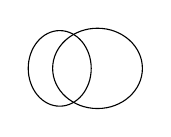
\begin{tikzpicture}[baseline=0cm]
\draw (0,0) ellipse (0.40cm and 0.48cm);
\draw (0.48,0) ellipse (0.57cm and 0.51cm);
\end{tikzpicture}
\end{adjustbox}
\quad $U\subset\mathbb H^n$, $V\subset\mathbb H^n$.
\begin{equation*}
f:U\to V.
\end{equation*}
\begin{equation*}
\forall x\in U\quad df_x:\mathbb H^n\to\mathbb H^n
\tag{1}
\end{equation*}
морфизм левых модулей
([зачёркнуто: \Unclear{GELFAND-P001371}{morphism-cancellation}{матр.?}]
умн. на матр. справа).

Если оно односвязно, то получится только линейное пр-во.
[Под строкой: открывающая скобка без продолжения.]

Все автоморфизмы линейны.

Можно написать алг. Ли инфинитезим. преобразований, которые её сохраняют.

(2) \underline{Утв.}: тогда ф-и перехода будут обязательно линейными.

1-е приближение \Unclear{GELFAND-P001371}{approximation-ending}{тривиальн.?}.

Вект. поле, у к-рого дифференциал — кватернионная матрица
[зачёркнуто: \Unclear{GELFAND-P001371}{matrix-cancellation}{неразборчивый знак}].

\underline{Опр-е (1) неверно}, т.к. тогда проективное пр-во не будет
иметь кватернионную структуру.

$\mathbb C P^n$ — пр-во 1-мерных кватернионных подпр-в в $\mathbb H^{n+1}$.

$\mathbb C P^1$ — пары $(\lambda_1,\lambda_2)$ с точн. до левого умн.
$(\lambda\lambda_1,\lambda\lambda_2)$.
\Unclear{GELFAND-P001371}{projective-space-letter}{В обозначениях проективных пространств видна буква $\mathbb C$.}

2 карты \quad $(\lambda_1,1)$,\quad $(1,\lambda_2)$.
\begin{equation*}
(\lambda_1,1)\sim(1,\lambda_1^{-1}).
\end{equation*}
$\lambda\to\lambda^{-1}$ — функция перехода.

\SourcePage{GELFAND-P001372}{50}
$\lambda^{-1}$
\begin{equation*}
(\lambda_0+i\lambda_1+j\lambda_2+k\lambda_3)^{-1}
=\frac{\lambda_0-i\lambda_1-j\lambda_2-k\lambda_3}
{\lambda_0^2+\lambda_1^2+\lambda_2^2+\lambda_3^2}.
\end{equation*}
\begin{equation*}
d(\lambda^{-1})=-\lambda^{-1}d\lambda\,\lambda^{-1}.
\end{equation*}

\underline{Топ. объяснение}: если бы было, то на $S^3$ было бы 3 комплексных структуры.

$V=\mathbb R^{4n}$.

(3) \underline{Кватернионная структура} — подалгебра $Q\subset$
[зачёркнуто: \Unclear{GELFAND-P001372}{endomorphism-cancellation}{неразборчивый знак}]
$\operatorname{End}(V)$, изоморфная $\mathbb H$.

(Или подалг., натянутая на 3 антикоммутир. компл. структуры
\begin{equation*}
Q=\langle I,J,K,E\rangle,\qquad
I^2=J^2=K^2=-1,\quad IJ=-JI=K
\end{equation*}
и т.д.

$\Rightarrow$ можно умножать слева на кватернионы.

\underline{Иначе}: изоморфизм не фиксирован; не надо выделять $I$, $J$ и $K$.

($\mathbb H$ имеет нетривиальные автоморфизмы.)

\underline{Кватернионная структура} на мн-зии: поле кватернионных структур
(в каждом касательном пр-ве). (Или: почти кватерн. структура.)

Chern (1945) рассматривал такие.

($\forall$ 4-мерн. рим. мн-зие обладает двумя, т.к.
$\operatorname{SO}(4)=\text{произвед.}$

$M^{4n}$, $Q:x\mapsto Q_x$.

\underline{Интегрируемость}: вместо атласа — ур-я Коши--Римана.

(С точн. до малых 2-го порядка
[зачёркнуто: \Unclear{GELFAND-P001372}{integrability-cancellation}{неразборчивое слово}]
как кватернионное преобр.)

\underline{Автоморфизмы, сохр. кватерн. структуру}
\begin{equation*}
G=\operatorname{GL}(1,\mathbb H)\cdot\operatorname{GL}(n,\mathbb H)
\qquad\text{— гр. автом. кватернионной структ.}
\end{equation*}
\begin{equation*}
G=\operatorname{Sp}(1)\cdot\operatorname{Sp}(n)
\end{equation*}
— для [зачёркнуто:
\Unclear{GELFAND-P001372}{sp-word-cancellation}{обычного?}]
опред. (1).
[Над зачёркнутым словом также зачёркнуто:
\Unclear{GELFAND-P001372}{sp-upper-cancellation}{неразборчивый знак}.]
\Unclear{GELFAND-P001372}{automorphism-groups}{Группы и ссылка на опред. (1) переданы буквально.}

\begin{equation*}
y_i=\sum x_k a_{ki}
\end{equation*}
[Между $\sum$ и $x_k$ зачёркнуто:
\Unclear{GELFAND-P001372}{summation-cancellation}{неразборчивый символ}.]
$\Vert$ сохр. кватерн. структуру (правую).
\Unclear{GELFAND-P001372}{right-structure}{Слово «правую» сохранено.}

\begin{equation*}
(x_1,\ldots,x_n)\to(\lambda x_1,\ldots,\lambda x_n)
\end{equation*}
тоже сохраняет.

[В правой скобке перед первой $\lambda$ зачёркнуто:
\Unclear{GELFAND-P001372}{tuple-first-cancellation}{$x_1$?};
между этой $\lambda$ и $x_1$ зачёркнуто:
\Unclear{GELFAND-P001372}{tuple-second-cancellation}{неразборчивый знак}.]

[Под формулой, со стрелкой к месту между первой $\lambda$ и $x_1$:]
(С другой стороны!)

\SourcePage{GELFAND-P001373}{unlabelled}
\underline{Условие 1-интегрируемости:}

$\exists$ связность $\nabla$ без кручения, сохр. кватернионную структуру.

(Лин. связность, не обяз. метрическая.)

[Зачёркнуто в скобках:
\Unclear{GELFAND-P001373}{cancelled-parenthesis}{неразборчивая фраза}.]
Или: $\nabla Q=0$.

Кватернионное подпр-во $\longrightarrow$ кватернионное подпр-во при пар. переносе.

[Разделительная черта.]

\underline{Гончаров А.}

Пусть есть вещ.-аналит. мн-зие с [вписано: почти] кватернионной структурой.
\begin{equation*}
M_{\mathbb R}^{4n}\subset M_{\mathbb C}^{4n}.
\end{equation*}
\begin{equation*}
T_xM_{\mathbb C}^{4n}\supset K_x
=\bigcup\{v+\sqrt{-1}\,Jv\},\qquad v\in TM_{\mathbb R}^{4n},
\end{equation*}
[Над $K_x$: конус.]
\begin{equation*}
J\in Q_x,\qquad J^2=-1.
\end{equation*}
И должна быть интегрируемость.

[Разделительная черта.]

Д.А.
\begin{equation*}
\gamma\text{ — кривая}\quad\Rightarrow\quad
\tau_\gamma Q_{\gamma(0)}=Q_{\gamma(1)}.
\end{equation*}
\begin{equation*}
\gamma:[0,1]\to M.
\end{equation*}
($\tau_\gamma$ — пар. перенос вдоль $\gamma$.)

$Q_x$ — подалгебра в $\operatorname{Aut}T_xM$,
её тоже можно переносить.
\Unclear{GELFAND-P001373}{algebra-in-aut}{В рукописи: «подалгебра в $\operatorname{Aut}T_xM$».}

\SourcePage{GELFAND-P001374}{unlabelled}
\underline{20/IV-87г.}\qquad\underline{Сем. Гельфанда.}

\underline{И.М.Г.} Вопрос: есть 2 коммутир. изометрии в $n$-мерном пр-ве;
[приписка над строкой с указателем: не всюду опр.]
как из них сделать 2 коммутир. унит. оператора? Какие препятствия?

Частично это сделано у Каспарова.

\underline{Кириллов о раб. Джонса.}

\underline{Различение}
[зачёркнуто: \Unclear{GELFAND-P001374}{knot-cancellation}{узлов?}]
\underline{узлов с помощью факторов.}

Рассм. алгебру, порождённую образ. $T_i$ (беск. числом) с соотношениями
\begin{equation*}
\begin{cases}
(T_i+1)(T_i-q)=0,\\
T_iT_{i+1}T_i=T_{i+1}T_iT_{i+1},\\
T_iT_j=T_jT_i,\quad |i-j|>1.
\end{cases}
\tag{1}
\end{equation*}
(Алг. Гекке серии $A$.)

$\Rightarrow$ [зачёркнуто:
\Unclear{GELFAND-P001374}{series-cancellation}{неразборчивый знак}]
в Ленинграде \Unclear{GELFAND-P001374}{leningrad-verb}{приложили?}
так же серию $B$.

1. Узел $\longrightarrow$ многочлен, эквив. узлы $\longrightarrow$ равные многочлены.

2. Фактор $\longrightarrow$ подфактор.

\SourcePage{GELFAND-P001375}{unlabelled}
Рассм. $\coprod_n B_n$
([зачёркнуто: \Unclear{GELFAND-P001375}{union-cancellation}{неразборчивое сокращение}]
дизъюнктное объединение).
[Под $B_n$ с указателем: гр. кос.]

\underline{Зацепление}: ориентир. 1-мерное комп. мн-зие, погруженное в $\mathbb R^3$.
\Unclear{GELFAND-P001375}{link-immersion}{В определении написано «погруженное».}

[Слева от схемы: \Unclear{GELFAND-P001375}{left-isolated-mark}{короткий изолированный штрих}.]

\SourceFigure{GELFAND-P001375}{braids-links-diagram}{Сверху $\coprod_n B_n$.
От него стрелка вниз-влево к $H$ и стрелка вправо-вниз к рисунку двух
перекрывающихся ориентированных петель. Слева от $H$ написано «фактор»;
под $H$ с коротким указателем — «алгебра Гекке (1)».
От $H$ стрелка вниз-вправо к слову «многочлены».
На рисунке петель обе видимые стрелки направлены вверх по правым ветвям;
верхние дуги бледны и прерваны, соединения и верхнее пересечение требуют проверки по скану.}

% Future-only, uncompiled partial ink recreation; no live frame replacement.
% P1375 original native diagram bbox [185,450,1445,960].
% Coordinates below are original scan pixels; Bézier centerlines are approximate.
% The topological connectivity and over/under order are intentionally unresolved.
% Existing frame prose and its seven literal Unclear calls are outside this fragment.
\ReaderDiagramPair{figures/gelfand-0149-p001375-braids-links-original.png}{GELFAND-P001375}{%
\begin{tikzpicture}[x=0.006cm,y=-0.006cm,line cap=round,line join=round,
  every node/.style={inner sep=1pt,font=\small}]
\path[use as bounding box] (185,450) rectangle (1445,960);
\node at (700,535) {$\coprod_n B_n$};
\node at (475,700) {$H$};
\node at (315,720) {фактор};
\node[align=center] at (435,874) {алгебра\\Гекке $(1)$};
\node at (825,910) {многочлены};
% Three directly visible directed connecting strokes.
\draw[->,line width=0.7pt] (593,595) -- (524,672);
\draw[->,line width=0.4pt] (805,545) -- (979,604);
\draw[->,line width=0.6pt] (563,757) -- (647,880);
% The lower-left shaft and separate bent stroke are kept separate.
% Neither a new arrowhead nor a reverse-directed arrow is inferred here.
\draw[line width=0.55pt] (451,752) -- (430,811);
\draw[line width=0.3pt] (441,815) -- (465,804) -- (472,813);
% Left visible curved strand: open at the upper left and at its right arrowhead.
\draw[line width=0.5pt] (1129,601)
  .. controls (1101,606) and (1075,639) .. (1082,674)
  .. controls (1088,716) and (1123,739) .. (1164,739);
\draw[line width=0.3pt] (1164,739)
  .. controls (1190,730) and (1219,692) .. (1221,657);
% Detached faint upper fragment, preserving the native visible gap.
\draw[line width=0.25pt] (1144,611)
  .. controls (1160,610) and (1186,613) .. (1199,622);
% A separate explicit visible upward arrowhead, with no inferred upper closure.
\draw[line width=0.45pt] (1196,685) -- (1221,655) -- (1235,682);
% Right visible curved strand: inner upper endpoint remains open.
% Its lower contact with the left curve is drawn without a vertex or underpass.
\draw[line width=0.8pt] (1166,648)
  .. controls (1155,677) and (1153,715) .. (1164,739)
  .. controls (1177,782) and (1215,803) .. (1240,801);
\draw[line width=0.35pt] (1240,801)
  .. controls (1298,806) and (1359,728) .. (1361,655);
% Separate upper arc; do not connect its left endpoint to the inner strand.
\draw[line width=0.45pt] (1210,600)
  .. controls (1250,562) and (1286,562) .. (1322,575);
\draw[line width=0.25pt] (1322,575)
  .. controls (1356,590) and (1358,624) .. (1361,651);
\draw[line width=0.45pt] (1335,674) -- (1361,651) -- (1378,684);
\end{tikzpicture}
}
\Unclear{GELFAND-P001375}{braids-links-connectivity}{Верхние разрывы двух кривых оставлены открытыми по видимому рисунку; их соединения и порядок над/под в нижнем соприкосновении не установлены.}
\Unclear{GELFAND-P001375}{hecke-indicator}{Под $H$ видны косой штрих и отдельный угловой штрих над подписью «алгебра Гекке (1)»; однозначное острие и направление указателя не установлены.}


Коса $\longrightarrow$ зацепление (соед. начало с концом).

Един. коса $\longrightarrow$
\begin{adjustbox}{max width=\linewidth}
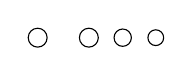
\begin{tikzpicture}[baseline=-0.1cm]
\draw (0,0) circle (0.12cm);
\draw (0.65,0) circle (0.12cm);
\draw (1.08,0) circle (0.11cm);
\draw (1.50,0) circle (0.10cm);
\end{tikzpicture}
\end{adjustbox}

(2) $b\subset B_n$ и $\widetilde b\subset B_n$ задают эквив. зацепления.
[Под $\widetilde b$:] $\widetilde b=cbc^{-1}$.
[Справа, за вертикальной чертой:] $B_n\subset B_{n+1}$.
\Unclear{GELFAND-P001375}{braid-membership}{В (2) перед $B_n$ стоят знаки, похожие на $\subset$.}

(3) $b\in B_n$, $\widetilde b\in B_{n+1}$,
$\widetilde b=b\cdot\sigma_n^{\pm1}$
(дописывание одной образ. из $B_{n+1}$).

Тогда $b$ и $\widetilde b$ порожд.
[зачёркнуто: \Unclear{GELFAND-P001375}{equivalence-cancellation}{экв.?}]
эквив. зацепления.

% Source diagram: bbox [385,1760,705,2150], original pixels.
\begin{adjustbox}{max width=\linewidth}
\begin{tikzpicture}[baseline=0cm]
\draw (-0.65,2) -- (1.50,2);
\fill (-0.65,2) circle (0.02cm);
\draw[->] (-0.65,0) -- (1.40,0);
\draw (0.80,2) .. controls (0.80,1.62) and (0.60,1.25) .. (0.37,1.12);
\draw (-0.03,0) .. controls (-0.03,0.38) and (0.16,0.66) .. (0.29,0.85);
\draw (0,2) .. controls (-0.06,0.90) and (0.80,1.10) .. (0.80,0);
\node[above] at (0,2) {$k$};
\node[above] at (0.80,2) {$k+1$};
\node[below] at (-0.03,0) {$k$};
\node[below] at (0.80,0) {$k+1$};
\node[right] at (1.03,1.03) {$\sigma_k$ — образующие};
\end{tikzpicture}
\end{adjustbox}

(4) \underline{Теор. Маркова} (трудная): опис. операции достаточны
для перехода к любому эквив. зацеплению.

Идея: построить инвариантную отн. этих операций ф-ю.

Отобр. $\coprod_n B_n$ в $H$ строится так:
$\sigma_i\to T_i$, $\sigma_i^{-1}\to T_i^{-1}$.
[К $T_i^{-1}$ снизу: найденное из квадр. ур-я $(1)_1$.]

$(1)_{2,3}$ — полный набор соотношений в группе кос.
\begin{equation*}
\sigma_i^{-1}\longrightarrow\frac{T_i+(1-q)}{q}=T_i^{-1}.
\end{equation*}

Набор образ. (1) [вписано: $\forall q$] имеет единственное фактор-представление
со следом, причём
[зачёркнуто: \Unclear{GELFAND-P001375}{trace-cancellation}{неразборчивый фрагмент}]
след — многочлен от $q$, $q^{-1}$.
\begin{equation*}
\mathbb Z[q,q^{-1}].
\end{equation*}
\Unclear{GELFAND-P001375}{factor-claim-parameter}{Приписка $\forall q$ и утверждение о единственности оставлены без дополнений.}

\SourcePage{GELFAND-P001376}{57}
\underline{Упражнение}. Взять $q=\pm1$ и посмотреть, какой здесь
получается инвариант группы кос (отношение значений многочлена
Джонса при этих значениях).

\underline{Джонс} специально исключал из рассмотрения
[зачёркнуто: \Unclear{GELFAND-P001376}{roots-cancellation}{неразборчивый фрагмент}]
корни из $1$.

\underline{Идея И.М.Г.}: рассмотреть именно корни из $1$.
Может оказаться, что факторов вообще нет, а нужно корни из $1$.

А.М. Вершик что-то уже сделал по этому поводу.

\paragraph*{\underline{А. Бейлинсон.}}
О раб. Бейлинсона, МакФерсона и В. Шехтмана.

\underline{Заметки о мотивных когомологиях}

Пусть $X$ — ан. мн-зие, $E$ — вект. расслоение на $X$.
[Под характеристикой $X$:] (или \Unclear{GELFAND-P001376}{x-parenthesis}{компл.?})
(компактное).
\begin{equation*}
c_i(E)\in H^{2i}(X,\mathbb C)
=H^{2i}(X,\mathcal O\to\Omega^1\to\ldots).
\end{equation*}
[Над последним аргументом, с указателем: когом. с коэфф. в комплексе пучков.]

Они целочисленны и удовл. усл. Ходжа
([зачёркнуто: \Unclear{GELFAND-P001376}{hodge-cancellation}{неразборчивое слово}]
$c_i\in i$-му члену фильтр. Ходжа).

(Т.к. можно вычислить через $\log$ произв. в коциклах Чеха.)

Будем вычислять когомологии мн-зия из компл. де Рама.
\begin{equation*}
(1)\qquad 0\to\mathbb C\to
\text{[зачёркнуто: }\Unclear{GELFAND-P001376}{de-rham-cancellation}{неразборчивый знак}\text{]}
\mathcal O\to\Omega^1\to\Omega^2\to\ldots
\end{equation*}
[Справа:] $\Omega^i$ — голом. $i$-формы (пучок).

$\{U_i\}$ — покрытие $X$ маленькими откр. мн-вами.

Сопоставим:
\begin{center}
$(*)\quad$
\begin{adjustbox}{max width=\linewidth}
\begin{tikzcd}
C^{2i}(\mathcal O)\arrow[r] & C^{2i}(\Omega^1) \\
 & C^{2i-1}(\Omega^1)\arrow[u]\arrow[r] & \ldots
\end{tikzcd}
\end{adjustbox}
\end{center}

Фильтрация Ходжа на $H^k(X,\mathbb C)$:
\begin{equation*}
F^j H^k(X,\mathbb C)
=H^k(X,0\to\ldots\to0\to\Omega^j\to\Omega^{j+1}\to\ldots).
\end{equation*}
\underline{Констр. Атьи хар. класса, из к-рой следует, что $c_j\in F^j$}.

$g_{ij}$ — ф-и переклейки.
\begin{equation*}
g_{ij}\colon U_i\cap U_j\longrightarrow GL_n(\mathbb C).
\end{equation*}
\begin{equation*}
A=g_{ij}^{-1}dg_{ij}\in
\Omega^1(U_i\cap U_j,\operatorname{Mat}_n(\mathbb C))
\in C^1(X,\Omega^1\otimes\operatorname{Mat}_n).
\end{equation*}
[Под $g_{ij}^{-1}dg_{ij}$: 1-форма со знач. в алг. Ли.]
\Unclear{GELFAND-P001376}{cochain-membership}{В формуле для $A$ сохранены два последовательных знака $\in$.}

Надо взять $(g_{ij}^{-1}dg_{ij})^k$ — коцепь со знач. в $k$-формах.
[Под степенью: (перемн. коцепей; закрывающая скобка не видна. Справа — двойная черта.]

Берём след $\operatorname{Tr}$ $\longrightarrow$ получ. форма с одной компонентой.

\SourcePage{GELFAND-P001377}{unlabelled}
\begin{equation*}
c_i(E)=\operatorname{Tr}(A^i).
\end{equation*}
[Справа:] $A^i$ — форма степ. $i$ на пересеч. $(i+1)$-го мн-ва.
\Unclear{GELFAND-P001377}{chern-trace}{Обозначение $c_i(E)$ перед следом степени сохранено.}

[Зачёркнуто: \Unclear{GELFAND-P001377}{element-cancellation}{Вид?}]
$\Rightarrow$ элемент $2i$-мерных когомологий (см. диагр. $(*)$).

\underline{Задача}: явно построить гомотопию в целочисл. хар. класс.

Для
\begin{equation*}
c_1=d\log(\det g_{ij}).
\end{equation*}

Надо отбросить $d$:
\begin{adjustbox}{max width=\linewidth}
\begin{tikzpicture}[baseline=0cm]
\node at (0,0) {$\log(\det g_{ij})$};
\node[right] at (1.3,0) {на малом мн-ве};
\node[rotate=-90] at (0,-0.60) {$\in$};
\node at (0,-1.15) {$C^1(\mathcal O)$};
\end{tikzpicture}
\end{adjustbox}

\SourcePage{GELFAND-P001378}{unlabelled}
\underline{27.4.87 г.}\qquad \underline{Сем. Гельфанда}

\paragraph*{\underline{А. Бейлинсон}}
\underline{Когомологии Делиня} [над концом заголовка вписано: — Бейлинсона]:
см. \Unclear{GELFAND-P001378}{soule-reference}{обз.?} Soulé,
сем. Бурбаки, фев. 85.
[Под фамилией:] (Regulateurs).

\underline{H. Esnault, E. Viehweg} (препринт).
[Под словом «препринт»: есть у Манина.]

Deligne--Beilinson cohomology

\underline{Бейлинсон}: Совр. пробл. матем. т. 24.

Contempor. math. \Unclear{GELFAND-P001378}{bibliography-number}{$\sim$ № 25?}

\underline{Комплекс пучков} на любом мн-зии (компл. аналитич. схем).
\begin{equation*}
(1)\qquad
\mathbb Z(i)_{\mathcal D}:=
\mathbb Z\overset{(2\pi\sqrt{-1})^i}{\longrightarrow}
\mathcal O\longrightarrow\Omega^1\longrightarrow\ldots
\longrightarrow\Omega^{i-1}.
\end{equation*}

($i$ — целое.)

В частности
\begin{equation*}
\mathbb Z(0)_{\mathcal D}=\mathbb Z,
\end{equation*}
\begin{equation*}
\mathbb Z(1)_{\mathcal D}=
\bigl(\mathbb Z\overset{2\pi\sqrt{-1}}{\longrightarrow}\mathcal O\bigr)
\overset{\exp}{\longrightarrow}\mathcal O^*[-1].
\end{equation*}
[Под $\mathcal O^*$ скобка и подпись: степ. 1.]

[Справа:]
\begin{adjustbox}{max width=\linewidth}
\begin{tikzcd}
\mathbb Z\arrow[r]\arrow[d] & \mathcal O\arrow[d,"\exp"] \\
0\arrow[r] & \mathcal O^*
\end{tikzcd}
\end{adjustbox}

[Под диаграммой:] морф. комплексов.

Пучок когом. есть
\begin{equation*}
H^1(\mathbb Z(1))=\mathcal O^*.
\end{equation*}
\begin{equation*}
\mathbb Z(2)_{\mathcal D}=
\bigl(\mathbb Z\overset{-4\pi^2}{\longrightarrow}\mathcal O
\longrightarrow\Omega^1\bigr).
\end{equation*}
\begin{equation*}
H^1(\mathbb Z(2)_{\mathcal D})=
\mathbb C/(2\pi\sqrt{-1})^2\mathbb Z.
\end{equation*}
[Под правой частью:]
\begin{adjustbox}{max width=\linewidth}
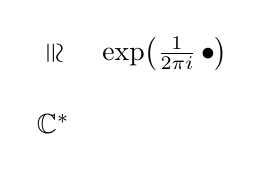
\begin{tikzpicture}[baseline=0cm]
\node[rotate=-90] at (0,0) {$\cong$};
\node[right] at (0.5,0) {$\exp\bigl(\frac{1}{2\pi i}\,\bullet\bigr)$};
\node at (0,-0.9) {$\mathbb C^*$};
\end{tikzpicture}
\end{adjustbox}
\Unclear{GELFAND-P001378}{exponential-placeholder}{Последний знак в аргументе экспоненты похож на точку или кружок.}

\begin{equation*}
H^2(\mathbb Z(2)_{\mathcal D})=\Omega^1/d\mathcal O.
\end{equation*}
\SourcePage{GELFAND-P001379}{67}
имеется отобр
\begin{equation*}
\mathbb{Z}(i)_{\mathcal D}\longrightarrow\mathbb{Z}
\qquad\text{(0-я компонента)}\tag{2}
\end{equation*}
\begin{equation*}
\mathbb{Z}(i)_{\mathcal D}\longrightarrow\Omega^i[-i]\tag{3}
\end{equation*}
(0 на всех формах, последняя — в ее дифференциал)
\begin{equation*}
\mathbb{Z}(i)_{\mathcal D}\otimes\mathbb{Z}(j)_{\mathcal D}
\longrightarrow\mathbb{Z}(i+j)_{\mathcal D}\tag{4}
\end{equation*}
\begin{equation*}
z_i\star\omega_j=z_i\omega_j
\end{equation*}
[Справа от (4):] стрелки (2) и (3) переводят это умн. в обычное умн. на числах и формах.

Пусть $z_j$ из 0-й комп.
\begin{equation*}
z_1\star z_2=z_1z_2\qquad\text{(обычное произв-е.)}\tag{5'}
\end{equation*}
\begin{equation*}
z_1\star\omega_2=z_1\omega_2\tag{5''}
\end{equation*}
\begin{equation*}
\omega_1\star z_2=z_2\omega_1\tag{5'''}
\end{equation*}
\begin{equation*}
\omega_1\star\omega_2=
\begin{cases}
0, & \text{если }\omega_2\notin\Omega^{j-1},\\
\omega_1\wedge d\omega_2, & \text{если }\omega_2\in\Omega^{j-1}
\end{cases}\tag{6}
\end{equation*}
(7) С точн. до \underline{гомотопии} это умн. коммутативно.
[Под «гомотопии»: (цепных комплексов).]

(8) Оба отображения (2), (3) коммутируют с умножением.

(9) Пусть $E$ — голом. векторное расслоение [вставлено: на $X$]. Тогда определены его классы Черня
\begin{equation*}
c_i(E)\in H^{2i}(X,\mathbb{Z}(i)_{\mathcal D})
\end{equation*}
[Справа:] (гр. когом. с коэфф. в комплексе пучков).
[Над началом примечания приписано:
\Unclear{GELFAND-P001379}{eq09-insertion}{абелевых}.]

(10) При отобр. (2) они перейдут в обычные топ. классы Черня;
этим св-вом и св-вом функториальности эти кл. (9) опр. однозначно.

\underline{Описание группы} $H^{2i}(X,\mathbb{Z}(i)_{\mathcal D})$.

Пусть $X$ компактно.

Определение когом. в (9) по Чеху.

$C^{ij}$ — $i$-мерные коцепи с коэфф. в $j$-м пучке.

[Слева от схемы зачеркнуто:
\Unclear{GELFAND-P001379}{cochain-cancellation}{неразборчивый знак}.]
\begin{equation*}
\begin{adjustbox}{max width=\linewidth}
\begin{tikzcd}[column sep=large,row sep=large]
C^{ij}\arrow[r,"d"]\arrow[dr,"\delta"'] & C^{i,j+1}\\
& C^{i+1,j}
\end{tikzcd}
\end{adjustbox}
\end{equation*}
[Справа:] $d$ — дифф. в комплексе (де Рам).

Теперь для $d+\delta$ нас есть обычные когомологии.

(Это получается при $C^*$ [зачеркнуто:
\Unclear{GELFAND-P001379}{bottom-cancellation}{неразборчивый знак}]
$X$ (целочисленные)).

\SourcePage{GELFAND-P001380}{unlabelled}
Для компактного $X$
\begin{equation*}
H^n(X,\mathbb{C})=\bigoplus_{a+b=n}H^{a,b}(X)
\qquad\text{(разл. Ходжа)}\tag{11}
\end{equation*}
\begin{equation*}
F^iH^n(X,\mathbb{C})=\bigoplus_{a\ge i}H^{a,b}
\qquad\text{(фильтрация Ходжа)}\tag{12}
\end{equation*}
Известно, что
\begin{equation*}
H^{a,b}(X)=H^b(X,\Omega^a)\tag{13}
\end{equation*}
Тогда
\begin{equation*}
\begin{gathered}
0\longrightarrow
\frac{H^{n-1}(X,\mathbb{C})}
{H^{n-1}(X,\mathbb{Z})+F^iH^{n-1}(X,\mathbb{C})}
\longrightarrow H^n\bigl(X,\mathbb{Z}(i)_{\mathcal D}\bigr)\\
\longrightarrow H^n(X,\mathbb{Z})\cap F^iH^n(X,\mathbb{C})\longrightarrow0
\end{gathered}\tag{14}
\end{equation*}
[В среднем члене (14), после $X,$ и перед $\mathbb Z(i)_{\mathcal D}$, зачеркнуто:
\Unclear{GELFAND-P001380}{eq14-cancellation}{неразборчивый знак}.]
Класс когомологий Делиня $\sim$ (разность целочисл. коцикла и коцикла де Рама) $+$ (соед. их гомотопия).

\underline{Коцепь с коэфф. в комплексе Делиня.}

Коцикл $\alpha$ [зачеркнут или переправлен нижний знак:
\Unclear{GELFAND-P001380}{cocycle-index}{неразборчиво}]
$\in Z^n(X;\mathbb{Z}(i)_{\mathcal D})$ состоит из набора
\begin{equation*}
\begin{cases}
\alpha_0\in Z^n(X,\mathbb{Z}),\\
\alpha_1\in C^{n-1}(X,\mathcal O),\\
\alpha_2\in C^{n-2}(X,\Omega^1),\\
\vdots\\
\alpha_i\in C^{n-i}(X,\Omega^{i-1}),
\end{cases}\tag{15}
\end{equation*}
согласованного в том смысле, что
\begin{equation*}
\begin{cases}
\alpha_0=\delta\alpha_1,\\
d\alpha_1=\delta\alpha_2,\\
\vdots\\
\delta\alpha_i=d\alpha_{i-1}
\end{cases}\tag{16}
\end{equation*}
Отсюда
\begin{equation*}
d\alpha_i\in Z^{n-i}(X,\Omega^{i,\mathrm{cl}})
\qquad\text{(со знач. в замкн. формах)}\tag{17}
\end{equation*}
Поэтому можно рассмотреть
\begin{equation*}
\alpha_0-d\alpha_i\in Z^n(X,\Omega^\bullet)\tag{18}
\end{equation*}
(Остальное — гомотопия, \Unclear{GELFAND-P001380}{bottom-abbreviation}{устанавл.}

\SourcePage{GELFAND-P001381}{unlabelled}
[Номер справа вверху: \Unclear{GELFAND-P001381}{page-label}{68 / 62}.]

$\alpha_1+\alpha_2+\ldots+\alpha_i$
[зачеркнуто: \Unclear{GELFAND-P001381}{top-cancellation}{неразборчиво}]
$\in C$.
\begin{equation*}
d(\alpha_0+\alpha_1+\ldots+\alpha_i)=\alpha_0-d\alpha_i\tag{19}
\end{equation*}
\Unclear{GELFAND-P001381}{eq19-first-index}{В скобках первый индекс читается как $0$; в строке выше сумма начинается с $\alpha_1$.}

Пока это общие вещи в $\forall$ двойном комплексе.

(см. также раб. Габриэлова, Гельфанда и Лосика)

Опишем гр. $H^{2i}(X,\mathbb{Z}(i)_{\mathcal D})$ исходя из (14).
\begin{equation*}
\begin{gathered}
0\longrightarrow
\underbrace{\frac{H^{2i-1}(X,\mathbb C)}{H^{2i-1}(X,\mathbb Z)+F^i}}_{\substack{\Vert\\ J^i}}
\longrightarrow H^{2i}(X,\mathbb Z(i)_{\mathcal D})\\
\longrightarrow
\underbrace{H^{2i}(X,\mathbb Z)\cap F^iH^{2i}(X,\mathbb C)}_{\substack{\Vert\\ \mathrm{Hg}^i(X,\mathbb Z)}}
\longrightarrow0
\end{gathered}\tag{20}
\end{equation*}
[Под $J^i$:] (компл. тор, называемый $i$-м якобианом Гриффитса).
\begin{equation*}
H^{2i-1}=F^i\oplus\overline F^{\,i}
\end{equation*}
$\Rightarrow$ отсюда компл. структура в $J^i$.

(21) \underline{Пример.}
\begin{equation*}
c_1(\mathcal E)=c_1(\det\mathcal E)
\end{equation*}
$g_{ij}$ — ф-и перехода расслоения
[зачеркнуто: \Unclear{GELFAND-P001381}{transition-cancellation}{неразборчивый знак перед $\mathcal E$}]
$\mathcal E$

(со знач. в $\mathbb C^*$).
\begin{equation*}
c_1(\mathcal E)\in H^2(X,\mathbb Z(1)_{\mathcal D})
\end{equation*}
\begin{equation*}
c_1(\mathcal E)_0\in Z^2(X,\mathbb Z)\tag{22}
\end{equation*}
[В (22) у $\mathcal E$ перед закрывающей скобкой зачеркнут или переправлен нижний знак:
\Unclear{GELFAND-P001381}{eq22-correction}{неразборчиво}.]
\begin{equation*}
c_1(\mathcal E)_1\in C^1(X,\mathcal O),\tag{23}
\end{equation*}
причем
\begin{equation*}
\delta[c_1(\mathcal E)_1]=c_1(\mathcal E)_0\tag{23'}
\end{equation*}
(24) $c_1(\mathcal E)_1=$
\Unclear{GELFAND-P001381}{eq24-factor}{$\log(\operatorname{deg}g_{ij})$ / $\log(\det g_{ij})$}
— любое опрд. $\log$.

($c_1(\mathcal E)_0$ — нах. из (23')
[зачеркнуто: \Unclear{GELFAND-P001381}{eq24-comment-cancellation}{неразборчивый знак}]
и задаёт рассогласование).

Получается изоморф.
\begin{equation*}
c_1:\operatorname{Pic}(X)\overset{\sim}{\longrightarrow}H^2(X,\mathbb Z(1)_{\mathcal D})\tag{25}
\end{equation*}

\SourcePage{GELFAND-P001382}{unlabelled}
\underline{Построение $c_2$} (это уже связано с дилогарифмом).

$c_1$ строилось в 2 шага
\begin{equation*}
\mathcal E\overset{\det}{\longmapsto}
c_{1\,\mathrm{alg}}(\mathcal E)\in H^1(X,\mathcal O^*)
\overset{\text{«}\log\text{»}}{\longrightarrow}
H^2(X,\mathbb Z(1)_{\mathcal D})\tag{26}
\end{equation*}
В принципе должно было бы быть
\begin{equation*}
\begin{gathered}
c_i:\mathcal E\longmapsto
\underset{\substack{\Vert\\c_{iM}(\mathcal E)\\\text{(мотивные)}}}{c_{i\,\mathrm{alg}}(\mathcal E)}
=H^{2i}(X,\mathbb Z(i)_M)\\
\underset{\substack{\uparrow\\\text{полилогарифм}}}{\overset{\mathcal L i_i}{\longrightarrow}}
H^{2i}(X,\mathbb Z(i)_{\mathcal D})
\end{gathered}\tag{27}
\end{equation*}
\Unclear{GELFAND-P001382}{eq27-equality}{Между $c_{i\,\mathrm{alg}}(\mathcal E)$ и $H^{2i}$ в источнике стоит $=$.}

С точн. до кручения эта теория существует.

[Зачеркнуто: \Unclear{GELFAND-P001382}{before-vnei-cancellation}{неразборчиво}.]
в ней $\mathbb Z(1)_M=\mathcal O^*[-1]$.

\underline{Несколько требований.}

(28) а) $\mathbb Z(\text{отр. число})_M=0$

б) $\mathbb Z(0)_M=\mathbb Z$

в) $\mathbb Z(1)_M=\mathcal O^*[-1]$

г)
\begin{equation*}
\mathbb Z(2)_M=(\mathbb Z(2)_M^1\longrightarrow
\underset{\substack{\Vert\\\wedge^2(\mathcal O^*)}}{\mathbb Z(2)_M^2}
\qquad\text{(с точн. до 2-кручения)}
\end{equation*}
\Unclear{GELFAND-P001382}{eq28-parenthesis}{После второго члена внешняя круглая скобка не видна.}
\begin{equation*}
i\ge1:\ H^j(\mathbb Z(i)_M)=0\quad\text{при }j\notin[1,i]\tag{29}
\end{equation*}
\begin{equation*}
H^i(\mathbb Z(i)_M)=\mathcal K_i^{\mathrm{Milnor}}
\qquad\text{(пучок $K$-функторов Милнора)}\tag{30}
\end{equation*}
\underline{$K$-функтор Милнора.}

Для гладкого мн-зия (алгебраич.) это пучки.

(31) а) $\mathcal K_0^{\mathrm{Mil}}=\mathbb Z$,

б) $\mathcal K_1^{\mathrm{Mil}}=\mathcal O^*$.

в) [На левом поле: (соотн. Стейнберга).]
пусть $t\in\mathcal O^*$ и $1-t\in\mathcal O^*$, тогда
\begin{equation*}
\overset{\substack{\text{символ Стейнберга}\\\swarrow}}
{\underbrace{\{t,1-t\}}_{\text{произвед. в алгебре Милнора}}}=0
\end{equation*}
\Unclear{GELFAND-P001382}{milnor-degree}{$\mathcal K_0^{\mathrm{Mil}}$ / $\mathcal K_\circ^{\mathrm{Mil}}$ / $\mathcal K_\bullet^{\mathrm{Mil}}$}
$=$ своб. градуир. алгебра с обр.
[зачеркнуто: $\mathcal O^*$]
$\mathcal O^*=\mathcal K_1^{\mathrm{Mil}}$ и соотн. Стейнберга.

$\{ab,c\}=$ [зачеркнуто:
\Unclear{GELFAND-P001382}{bottom-product-cancellation}{$\{a,c\}\{b,c\}$ / $\{a,c\}+\{b,c\}$}]
$?$.

[Справа:] $\{\ \}$ — сложение.

\SourcePage{GELFAND-P001383}{69}
(32) Операция $\{\ \}$ суперкоммутативна в $\mathcal K^{\mathrm{Mil}}$.

В (28) г)

[На левом поле зачеркнут номер: \Unclear{GELFAND-P001383}{cancelled-number}{(33)?}.]
[Зачеркнута вся строка:
$\mathbb Z(2)_M^1=\mathbb Z[\mathbb P^1(X)]$.]
\begin{equation*}
\mathbb Z(2)_M^1=
\mathbb Z[(\mathbb P^1\setminus\{0,1,\infty\})(X)]/(\text{соотнош.})
\tag{33}
\end{equation*}
[От выражения с $\mathbb P^1$ вниз проведена линия к приписке:]
пучок ф-й на $X$, не приним. знач. $0,1,\infty$.

Дифференциал:
\begin{equation*}
\begin{aligned}
\mathbb Z(2)_M^1&\longrightarrow\mathbb Z(2)_M^2\\
t&\longmapsto t\wedge(1-t)
\end{aligned}\tag{34}
\end{equation*}
Соотношение из сообр., что лежит в ядре симв. Ст.

(5-чл. соотношение для дилогарифма)

Пусть $f,g$ — 2 ф-и, нигде не равные друг другу и не приним. значений $0,1,\infty$.
\begin{equation*}
(f,g,0,1,\infty)\tag{35}
\end{equation*}
(36) \underline{5 разных точек на} $\mathbb P^1$;
\underline{выбрасывая по 1-му, получим 5 двойных}
\underline{отнош. и надо взять их знакоперем.}
\Unclear{GELFAND-P001383}{eq36-abbreviation}{ф-ю};
это и есть 5-чл. соотн.

Вместо этого можно взять 5 независ. ф-й.

(37) \underline{Утв.} Соотн. (36) лежит в ядре дифференциала.

Впервые придумали Спенсер, Блох; Суслин установил связь с $K$-теорией.

Комплекс наз. комплексом Блоха — Суслина.

Надо построить отобр.
\begin{equation*}
\mathcal E\longmapsto c_2(\mathcal E)_M\in H^4(X,\mathbb Z(2)_M)\tag{38}
\end{equation*}
[В (38) между $c_2(\mathcal E)_M$ и знаком $\in$ зачеркнуто:
\Unclear{GELFAND-P001383}{eq38-cancellation}{неразборчивый математический фрагмент}.]

и ф-ю
\begin{equation*}
\mathbb Z(2)_M\longrightarrow\mathbb Z(2)_{\mathcal D}\tag{39}
\end{equation*}

\SourcePage{GELFAND-P001384}{unlabelled}
Построим отобр. (39).

(40)
\begin{equation*}
\begin{adjustbox}{max width=\linewidth}
\begin{tikzcd}[column sep=large,row sep=large]
&\mathbb Z(2)_M^1\arrow[r]\arrow[d,"\mathrm{dilog}"]
&\mathbb Z(2)_M^2\arrow[d]\\
\mathbb Z\arrow[r]&\mathcal O\arrow[r]&\Omega^1
\end{tikzcd}
\end{adjustbox}
\end{equation*}
[Справа от схемы:]
\begin{center}
\begin{adjustbox}{max width=\linewidth}
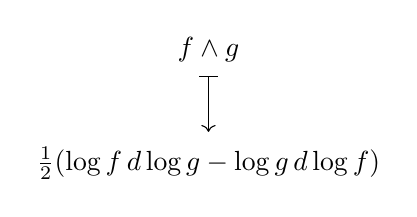
\begin{tikzpicture}
\node (upper) at (0,1.2) {$f\wedge g$};
\node (lower) at (0,-0.25) {$\frac12(\log f\,d\log g-\log g\,d\log f)$};
\draw[->] (0,0.85)--(0,0.15);
\draw (-0.12,0.85)--(0.12,0.85);
\end{tikzpicture}
\end{adjustbox}
\end{center}
\underline{Класс Черня.}
\begin{equation*}
\mathcal E\longmapsto c_2(\mathcal E)_M\in H^4(X,\mathbb Z(2)_M),\tag{41}
\end{equation*}
$\dim\mathcal E=2$, $\{U_i\}$, $s_i$ — сечение $\mathcal E$ над $U_i$.

2 компоненты.
\begin{equation*}
c_2(\mathcal E)_M^2\in C^2(\{U_i\},\mathbb Z(2)_M^2)
\end{equation*}
\begin{equation*}
c_2(\mathcal E)_M^1\in C^3(\{U_i\},\mathbb Z(2)_M^1)
\end{equation*}
$(s_1,\ldots,s_4)$ — 4 сечения $\mathcal E$.

Рассм. 4 точки $\mathbb P(\mathcal E)\ni s_1,\ldots,s_4$.

и т. д.

[Зачеркнуто: \Unclear{GELFAND-P001384}{bottom-cancellation}{двойное отнош.}.]

Строится с пом. двойного отношения.


\clearpage\section*{Полные примечания к чтению}
Ниже сохранены полные исторические наблюдения, варианты чтения и примечания к сверке. Указания увеличений описывают историческую работу с источником; сомнительные чтения здесь не объявляются разрешёнными.
\par

\subsection*{\texttt{GELFAND-P001359}}
\noindent\leavevmode\phantomsection\label{GELFAND-P001359:eq2-signs:note}\textbf{\texttt{GELFAND-0148-U001}} (eq2-signs).\par\nopagebreak[4]
Исходный PNG, координаты [x0,y0,x1,y1]=[470, 750, 1260, 1200], начало координат — левый верхний угол; В (1) перед 6uu\_x и u\_xxx стоят плюсы; в (2) написано ψ\_xx+uψ=k²ψ и ψ\_t=4ψ\_xxx+6uψ\_x+3u\_xψ. В (7), [400,2320,1160,2480], показатель ikx+4ik³t.\par
Варианты: Буквальная запись (1), (2), (7) с видимыми плюсами. Чтение в дипломатическом источнике остаётся неразрешённым.\par
При u=0 функция из (7) даёт ψ\_xx=−k²ψ и ψ\_t=+4ik³ψ, тогда как 4ψ\_xxx=−4ik³ψ. Это внутренняя математическая проверка, а не исправление источника. Противоречие знаков оставлено. Все области повторно просмотрены в увеличении 3×.\par\medskip
\noindent\leavevmode\phantomsection\label{GELFAND-P001359:eq3-overwriting:note}\textbf{\texttt{GELFAND-0148-U002}} (eq3-overwriting).\par\nopagebreak[4]
Исходный PNG, координаты [x0,y0,x1,y1]=[735, 1365, 1830, 1545], начало координат — левый верхний угол; В (3) первая K и следующая F обведены/правлены густыми штрихами. Между x и s, а также x и z заметны зачёркнутые плюсы с запятыми ниже.\par
Варианты: Первоначально F под конечной K и K под конечной F; Первоначальные буквы неразборчивы. Чтение в дипломатическом источнике остаётся неразрешённым.\par
Конечная запись K(x,s,t)F(s+z,t) и K(x,z,t) читается; нижний слой букв не восстановлен. Повторный просмотр 4×; перестановка букв не утверждается.\par\medskip
\noindent\leavevmode\phantomsection\label{GELFAND-P001359:after-eq8-cancelled:note}\textbf{\texttt{GELFAND-0148-U003}} (after-eq8-cancelled).\par\nopagebreak[4]
Исходный PNG, координаты [x0,y0,x1,y1]=[590, 2710, 740, 2840], начало координат — левый верхний угол; После «получим» и перед тире имеется короткая густо заштрихованная запись.\par
Варианты: ψ; неразборчивый зачёркнутый символ. Чтение в дипломатическом источнике остаётся неразрешённым.\par
Проверено увеличением 5×, исходный фрагмент [470,2690,795,2855]. Отдельные штрихи не позволяют уверенно восстановить отменённую запись.\par\medskip

\subsection*{\texttt{GELFAND-P001360}}
\noindent\leavevmode\phantomsection\label{GELFAND-P001360:eq11-coefficient:note}\textbf{\texttt{GELFAND-0148-U004}} (eq11-coefficient).\par\nopagebreak[4]
Исходный PNG, координаты [x0,y0,x1,y1]=[775, 575, 885, 700], начало координат — левый верхний угол; Перед ∂ψ/∂y в первой строке (11) стоит знак с маленькой верхней петлёй и пересечением нижних штрихов; он похож и на α, и на 2.\par
Варианты: α; 2. Чтение в дипломатическом источнике остаётся неразрешённым.\par
Повторно просмотрено 8×. В (10) и (12) читается α; это делает α контекстно вероятным, но не разрешает графическую неоднозначность (11). В формуле поставлен кандидат α с явным маркером, не исправление.\par\medskip
\noindent\leavevmode\phantomsection\label{GELFAND-P001360:before-eq13-short-cancelled:note}\textbf{\texttt{GELFAND-0148-U005}} (before-eq13-short-cancelled).\par\nopagebreak[4]
Исходный PNG, координаты [x0,y0,x1,y1]=[1260, 1480, 1385, 1570], начало координат — левый верхний угол; Между «по-другому» и «понимать» зачёркнуто короткое начало слова.\par
Варианты: об; оп; неразборчиво. Чтение в дипломатическом источнике остаётся неразрешённым.\par
Просмотрено в общем фрагменте [350,1475,1510,1630] при 4×. Прежняя запись не восстановлена.\par\medskip
\noindent\leavevmode\phantomsection\label{GELFAND-P001360:before-eq13-words-cancelled:note}\textbf{\texttt{GELFAND-0148-U006}} (before-eq13-words-cancelled).\par\nopagebreak[4]
Исходный PNG, координаты [x0,y0,x1,y1]=[355, 1540, 755, 1630], начало координат — левый верхний угол; Под строкой «Однако можно...» зачёркнуты два коротких слова; во втором заметна петля, похожая на Ф, и нижний вынос.\par
Варианты: как Фурье; по Фурье; неразборчивые два слова. Чтение в дипломатическом источнике остаётся неразрешённым.\par
Повторный просмотр 4×. Оба словесных кандидата предположительны; зачёркнутый текст не опущен молча.\par\medskip
\noindent\leavevmode\phantomsection\label{GELFAND-P001360:eq14-cancelled-argument:note}\textbf{\texttt{GELFAND-0148-U007}} (eq14-cancelled-argument).\par\nopagebreak[4]
Исходный PNG, координаты [x0,y0,x1,y1]=[1120, 1990, 1230, 2160], начало координат — левый верхний угол; В (14) между аргументами λ̄′ и λ имеется зачёркнутый символ, пересечённый несколькими наклонными штрихами.\par
Варианты: λ; χ; неразборчивый символ. Чтение в дипломатическом источнике остаётся неразрешённым.\par
Повторно просмотрено 5× в [880,1920,1435,2160]. Разбор аргументов T не восстанавливает отменённый символ; он отмечен отдельно от конечной формулы.\par\medskip
\noindent\leavevmode\phantomsection\label{GELFAND-P001360:eq15-overwritten-argument:note}\textbf{\texttt{GELFAND-0148-U008}} (eq15-overwritten-argument).\par\nopagebreak[4]
Исходный PNG, координаты [x0,y0,x1,y1]=[550, 2320, 620, 2415], начало координат — левый верхний угол; В левой части (15) второй аргумент K густо наведён. Виден конечный z, но под ним имеются дополнительные штрихи.\par
Варианты: z поверх x; повторно наведённое z. Чтение в дипломатическом источнике остаётся неразрешённым.\par
Повторно просмотрено 6× в [460,2300,665,2445]. Конечный z сохранён; первоначальная запись не утверждается.\par\medskip

\subsection*{\texttt{GELFAND-P001361}}
\noindent\leavevmode\phantomsection\label{GELFAND-P001361:heading-ending:note}\textbf{\texttt{GELFAND-0148-U009}} (heading-ending).\par\nopagebreak[4]
Исходный PNG, координаты [x0,y0,x1,y1]=[1310, 525, 1545, 615], начало координат — левый верхний угол; Последнее слово подчёркнутого заголовка после d-bar имеет окончание, в котором трудно отделить последний штрих ч от дополнительного и.\par
Варианты: задач.; задачи.. Чтение в дипломатическом источнике остаётся неразрешённым.\par
Повторно просмотрено 4× в [355,410,1555,640]. Грамматическая предпочтительность множественного числа не принимается за разрешение графического сомнения.\par\medskip
\noindent\leavevmode\phantomsection\label{GELFAND-P001361:eq21-cancelled:note}\textbf{\texttt{GELFAND-0148-U010}} (eq21-cancelled).\par\nopagebreak[4]
Исходный PNG, координаты [x0,y0,x1,y1]=[385, 1870, 985, 2005], начало координат — левый верхний угол; Слева от конечного коммутатора (21) зачёркнут коммутатор двух K с аргументами λ и η и знак равенства с последней цифрой. Нижние индексы пересечены штрихами.\par
Варианты: [K\_i(λ),K\_i(η)]=0; [K\_i(λ),K\_j(η)]=0. Чтение в дипломатическом источнике остаётся неразрешённым.\par
Просмотрено 5×. В обоих K наиболее заметен индекс, похожий на i; замена второго на j по аналогии с конечной формулой не утверждается.\par\medskip
\noindent\leavevmode\phantomsection\label{GELFAND-P001361:time-coefficient:note}\textbf{\texttt{GELFAND-0148-U011}} (time-coefficient).\par\nopagebreak[4]
Исходный PNG, координаты [x0,y0,x1,y1]=[625, 1075, 1010, 1220], начало координат — левый верхний угол; В третьей строке (19) виден коэффициент −4 без i; то же в экспоненте (20) [1510,1310,1810,1450] и I\_3=4λ³ в (23) [1135,2400,1420,2530].\par
Варианты: −4(λ³−η³) в (19), (20); I\_3=4λ³ в (23). Чтение в дипломатическом источнике остаётся неразрешённым.\par
Все три области просмотрены 3×. Формулы (19), (20), (22), (23) согласованы друг с другом, но связь временной нормировки с (7), (14) и заявленной КП (12) требует отдельной проверки. Фактор i по математическому ожиданию не добавлялся.\par\medskip
\noindent\leavevmode\phantomsection\label{GELFAND-P001361:eq24-cancelled-argument:note}\textbf{\texttt{GELFAND-0148-U012}} (eq24-cancelled-argument).\par\nopagebreak[4]
Исходный PNG, координаты [x0,y0,x1,y1]=[790, 2880, 865, 2970], начало координат — левый верхний угол; После открывающей скобки χ\_0 и до x,y,t густо зачёркнут дополнительный аргумент.\par
Варианты: λ; η; неразборчивый аргумент. Чтение в дипломатическом источнике остаётся неразрешённым.\par
Повторно просмотрено 6× в [700,2850,1030,2990]. Оставшиеся аргументы x,y,t читаются; отменённый знак не восстановлен.\par\medskip
\noindent\leavevmode\phantomsection\label{GELFAND-P001361:eq25-cancelled-word:note}\textbf{\texttt{GELFAND-0148-U013}} (eq25-cancelled-word).\par\nopagebreak[4]
Исходный PNG, координаты [x0,y0,x1,y1]=[1460, 3225, 1630, 3345], начало координат — левый верхний угол; Между «удовлетворяет» и «ур-ю» зачёркнуто короткое слово/сокращение с нижним выносом первой буквы.\par
Варианты: ф-ле; ф-и; неразборчиво. Чтение в дипломатическом источнике остаётся неразрешённым.\par
Просмотрено 6×. Предполагаемое «ф-ле» не утверждается как установленное чтение.\par\medskip

\subsection*{\texttt{GELFAND-P001362}}
\noindent\leavevmode\phantomsection\label{GELFAND-P001362:eq28-caption-ending:note}\textbf{\texttt{GELFAND-0148-U014}} (eq28-caption-ending).\par\nopagebreak[4]
Исходный PNG, координаты [x0,y0,x1,y1]=[1950, 1060, 2315, 1160], начало координат — левый верхний угол; Последнее слово подписи под f\_i(λ), после «с свобод. движущими», оканчивается сгущением штрихов, похожим на «ов»; начало «полюс» читается.\par
Варианты: полюсов; полюсами. Чтение в дипломатическом источнике остаётся неразрешённым.\par
Повторный просмотр 4× в [1200,1010,2325,1170]. Грамматически ожидаемое «полюсами» не подставлено вместо возможного «полюсов». Текст заканчивается до края изображения, это не утрата края.\par\medskip
\noindent\leavevmode\phantomsection\label{GELFAND-P001362:eq32-matrix-a:note}\textbf{\texttt{GELFAND-0148-U015}} (eq32-matrix-a).\par\nopagebreak[4]
Исходный PNG, координаты [x0,y0,x1,y1]=[2150, 2700, 2335, 2850], начало координат — левый верхний угол; В матрице A оба внедиагональных знака имеют наклонную верхнюю часть и нижнюю горизонталь; отдельная точка i неотчётлива и смешивается с сеткой. Рядом явно написано A²=−1.\par
Варианты: A=((0,i),(i,0)); A=((0,1),(1,0)). Чтение в дипломатическом источнике остаётся неразрешённым.\par
Матрицы просмотрены 8×, верхний правый элемент дополнительно 10× в [2220,2700,2305,2790]. Вариант i даёт A²=−1 и вместе с I=diag(1,−1) выполняет IA+AI=0; вариант 1 даёт A²=+1. Проверка поддерживает i, но не разрешает графического сомнения. Кандидат i в теле явно помечен. Для указанных абстрактных тождеств I²=1, A²=−1 и IA+AI=0 коммутатор M\_1,M\_2 из примера обращается в ноль; никакая исправленная матрица не утверждается.\par\medskip

\subsection*{\texttt{GELFAND-P001363}}
\noindent\leavevmode\phantomsection\label{GELFAND-P001363:after-diagram-verb:note}\textbf{\texttt{GELFAND-0148-U016}} (after-diagram-verb).\par\nopagebreak[4]
Исходный PNG, координаты [x0,y0,x1,y1]=[465, 700, 1170, 815], начало координат — левый верхний угол; Слово между «и затем» и «строить» имеет слитное окончание; основа «оста…» читается.\par
Варианты: остаётся; осталось. Чтение в дипломатическом источнике остаётся неразрешённым.\par
Просмотрено 5×. Ни грамматическая правка, ни уверенное прочтение окончания не внесены.\par\medskip
\noindent\leavevmode\phantomsection\label{GELFAND-P001363:eq34-number:note}\textbf{\texttt{GELFAND-0148-U017}} (eq34-number).\par\nopagebreak[4]
Исходный PNG, координаты [x0,y0,x1,y1]=[90, 1070, 255, 1245], начало координат — левый верхний угол; Слева от формулы читается (34), поверх цифр имеются наклонные и нисходящие штрихи.\par
Варианты: (34), номер обведён; (34), номер зачёркнут или исправлен. Чтение в дипломатическом источнике остаётся неразрешённым.\par
Просмотрено 7×. Значение 34 сохранено; назначение добавочных штрихов не установлено.\par\medskip
\noindent\leavevmode\phantomsection\label{GELFAND-P001363:title-cancelled:note}\textbf{\texttt{GELFAND-0148-U018}} (title-cancelled).\par\nopagebreak[4]
Исходный PNG, координаты [x0,y0,x1,y1]=[1195, 1250, 1390, 1350], начало координат — левый верхний угол; В заголовке Мигдала после «Другой смысл» перед «вычисления» короткое начало перечёркнуто несколькими горизонтальными штрихами.\par
Варианты: по; под; неразборчиво. Чтение в дипломатическом источнике остаётся неразрешённым.\par
Заголовок просмотрен 4× в [855,1200,2190,1390]. «матричных» вставлено над строкой; конечное «континуальным» проверено 6×.\par\medskip
\noindent\leavevmode\phantomsection\label{GELFAND-P001363:analog-phrase:note}\textbf{\texttt{GELFAND-0148-U019}} (analog-phrase).\par\nopagebreak[4]
Исходный PNG, координаты [x0,y0,x1,y1]=[925, 1395, 1480, 1515], начало координат — левый верхний угол; После «Некоммутирующий аналог» два слова; первое похоже на «символа», второе начинается прописным К и имеет очертания «Карасева».\par
Варианты: символа Карасева; смысла Карасева. Чтение в дипломатическом источнике остаётся неразрешённым.\par
Строка просмотрена 5×, фамилия 8× в [1050,1400,1480,1505]. Контекстом или внешней биографической информацией чтение не подменено. При заключительной сверке фамилия сопоставлена с ясным «способ Карасева» на GELFAND-P001366; неуверенность в предшествующем слове остаётся.\par\medskip
\noindent\leavevmode\phantomsection\label{GELFAND-P001363:eq3-cancelled-brackets:note}\textbf{\texttt{GELFAND-0148-U020}} (eq3-cancelled-brackets).\par\nopagebreak[4]
Исходный PNG, координаты [x0,y0,x1,y1]=[1090, 2120, 1195, 2340], начало координат — левый верхний угол; После e\textasciicircum{}\{At\} в (3) виден высокий зачёркнутый знак, похожий на закрывающую скобку, возможно с дополнительной круглой скобкой.\par
Варианты: ]; ]); неразборчивые скобки. Чтение в дипломатическом источнике остаётся неразрешённым.\par
Просмотрено 8×. Окончательные внешние круглые и квадратные скобки воспроизведены по правой части строки; зачёркнутый материал описан отдельно.\par\medskip

\subsection*{\texttt{GELFAND-P001364}}
\noindent\leavevmode\phantomsection\label{GELFAND-P001364:top-name:note}\textbf{\texttt{GELFAND-0148-U021}} (top-name).\par\nopagebreak[4]
Исходный PNG, координаты [x0,y0,x1,y1]=[500, 0, 955, 165], начало координат — левый верхний угол; В скобках после «И. М. Г. Зад.» написаны инициал Т. и фамилия с началом «Алекс…» и окончанием «…вская»; две средние гласные слитны.\par
Варианты: Т. Алексеевская; Т. Алексиевская. Чтение в дипломатическом источнике остаётся неразрешённым.\par
Просмотрено 6×. Фамилия не восстановлена из сведений о семинаре; исходная запись сохранена как кандидаты.\par\medskip
\noindent\leavevmode\phantomsection\label{GELFAND-P001364:top-parenthesis:note}\textbf{\texttt{GELFAND-0148-U022}} (top-parenthesis).\par\nopagebreak[4]
Исходный PNG, координаты [x0,y0,x1,y1]=[960, 0, 1275, 160], начало координат — левый верхний угол; После фамилии в отдельных скобках находится короткое слово с неясным первым сочетанием и окончанием, похожим на «…лал» или «…лан».\par
Варианты: сделал; сделала; сделан; неразборчиво. Чтение в дипломатическом источнике остаётся неразрешённым.\par
Просмотрено 6×. Эта помета относится к видимому верхнему блоку, а не добавлена из каталога. Число ответа 96 проверено отдельно 8× в [600,305,755,435].\par\medskip
\noindent\leavevmode\phantomsection\label{GELFAND-P001364:eq3-prime-cancelled:note}\textbf{\texttt{GELFAND-0148-U023}} (eq3-prime-cancelled).\par\nopagebreak[4]
Исходный PNG, координаты [x0,y0,x1,y1]=[860, 850, 1035, 1070], начало координат — левый верхний угол; Между 1/N² и частной производной стоит перечёркнутое нагромождение двух узких знаков; возможно, прежнее tr.\par
Варианты: tr; неразборчиво. Чтение в дипломатическом источнике остаётся неразрешённым.\par
Просмотрено 8×. Верхние ji у экспоненты в (3′) и нижние ji,jj,ii в (8) переданы по их расположению, без унификации индексов.\par\medskip
\noindent\leavevmode\phantomsection\label{GELFAND-P001364:proof-verb:note}\textbf{\texttt{GELFAND-0148-U024}} (proof-verb).\par\nopagebreak[4]
Исходный PNG, координаты [x0,y0,x1,y1]=[1280, 1635, 1580, 1745], начало координат — левый верхний угол; В пояснении к произведению после «поочерёдно» сокращённое слово начинается «вы…» и заканчивается «…рг.» либо похожим сочетанием.\par
Варианты: выдерг.; неразборчиво. Чтение в дипломатическом источнике остаётся неразрешённым.\par
Просмотрено 7× и в контексте 5× [930,1620,2260,1755]. Возможное разговорное «выдерг.» не развёрнуто до полного слова и не заменено математическим объяснением.\par\medskip

\subsection*{\texttt{GELFAND-P001365}}
\noindent\leavevmode\phantomsection\label{GELFAND-P001365:top-cancelled:note}\textbf{\texttt{GELFAND-0148-U025}} (top-cancelled).\par\nopagebreak[4]
Исходный PNG, координаты [x0,y0,x1,y1]=[340, 0, 570, 195], начало координат — левый верхний угол; Под вставленным над строкой «Далее» перечёркнуто слово с высоким начальным штрихом и нисходящим штрихом в конце, похожее на «Теперь».\par
Варианты: Теперь; неразборчиво. Чтение в дипломатическом источнике остаётся неразрешённым.\par
Просмотрено 6×. Квадратная скобка слева от «Далее» и закрывающая скобка после (11) воспроизведены. Наличие плюса в экспоненте (11) проверено; знак не исправлен.\par\medskip
\noindent\leavevmode\phantomsection\label{GELFAND-P001365:jump-normalization:note}\textbf{\texttt{GELFAND-0148-U026}} (jump-normalization).\par\nopagebreak[4]
Исходный PNG, координаты [x0,y0,x1,y1]=[225, 2310, 1420, 2975], начало координат — левый верхний угол; В (17) Im f определено как 1/2·(f(x+i0)−f(x−i0)); i в знаменателе нет. В (19) разность квадратов равна 2 Im f·Re f.\par
Варианты: буквальное чтение: коэффициенты 1/2 и 2; особая неоговорённая нормировка Im и Re; возможная авторская неточность коэффициента или обозначения. Чтение в дипломатическом источнике остаётся неразрешённым.\par
Коэффициент (17) просмотрен 8× в [575,2320,775,2435]; (19) проверено по увеличению нижней полосы 3×. При обычном Re f=(f\_++f\_-)/2 определение (17) давало бы f\_+²−f\_-²=4 Im f Re f. Ни i, ни множитель 4 в текст не подставлены; источник может пользоваться иной нормировкой, явно на этой странице она не определена. Формула (16) также оставлена буквально.\par\medskip
\noindent\leavevmode\phantomsection\label{GELFAND-P001365:eq20-description:note}\textbf{\texttt{GELFAND-0148-U027}} (eq20-description).\par\nopagebreak[4]
Исходный PNG, координаты [x0,y0,x1,y1]=[410, 3000, 1880, 3135], начало координат — левый верхний угол; В строке (20) после f два тесно написанных слова или сокращения; затем «в лев… полуплоскост…». В «лев…» имеется сгущение наложенных штрихов.\par
Варианты: f аналитич. продолж. в левую полуплоскость; f полностью предст. в левой полуплоскости. Чтение в дипломатическом источнике остаётся неразрешённым.\par
Строка просмотрена 5×, части слов дополнительно 8× в [445,3010,870,3125] и [900,3010,1190,3125]. Уверенно различимы f, предлог «в» и основа «полуплоскост»; кандидаты остальной фразы не утверждаются. Не заменено ожидаемым свойством резольвенты.\par\medskip
\noindent\leavevmode\phantomsection\label{GELFAND-P001365:last-parenthesis:note}\textbf{\texttt{GELFAND-0148-U028}} (last-parenthesis).\par\nopagebreak[4]
Исходный PNG, координаты [x0,y0,x1,y1]=[1880, 3170, 2385, 3330], начало координат — левый верхний угол; В последней скобке после «это» короткое сокращение перед словом «матрица»; видны петля, верхняя черта и мелкие конечные штрихи.\par
Варианты: беск.; вещ.. Чтение в дипломатическом источнике остаётся неразрешённым.\par
Просмотрено 8×, вся строка 5×. Свойства матрицы A из предыдущих страниц не использованы для выбора чтения; противоречия не устранены.\par\medskip

\subsection*{\texttt{GELFAND-P001366}}
\noindent\leavevmode\phantomsection\label{GELFAND-P001366:eq23-radicand:note}\textbf{\texttt{GELFAND-0148-U029}} (eq23-radicand).\par\nopagebreak[4]
Исходный PNG, координаты [x0,y0,x1,y1]=[520, 1080, 1480, 1320], начало координат — левый верхний угол; В (23) перед корнем минус; под корнем (V′/(2λ))²−R. В предыдущем кадре в (15) R=f²−V′f/λ.\par
Варианты: буквальное чтение (23): минус R; возможная смена знака определения R либо ошибка источника. Чтение в дипломатическом источнике остаётся неразрешённым.\par
Минус перед корнем проверен 8× в [965,1100,1075,1235]: вертикальный штрих относится к сетке. Квадратное уравнение (15) с его записанным определением R даёт под корнем (V′/(2λ))²+R. В тело этот плюс не внесён. Рядом имеется выноска «полином подбирается!», адресованная R.\par\medskip
\noindent\leavevmode\phantomsection\label{GELFAND-P001366:eq24-asymptotic:note}\textbf{\texttt{GELFAND-0148-U030}} (eq24-asymptotic).\par\nopagebreak[4]
Исходный PNG, координаты [x0,y0,x1,y1]=[480, 1410, 1880, 1620], начало координат — левый верхний угол; После стрелки с нижним ω→∞ видны подряд 1/ω−M(ω)√((ω−a)(ω−b)); над второй частью подпись «(из вып. гран. условий)».\par
Варианты: вся правая часть относится к стрелке; условие f(ω)→1/ω, за которым отдельно дописан член с M. Чтение в дипломатическом источнике остаётся неразрешённым.\par
Просмотрено 3× в общей полосе [205,1070,2010,1630], сопоставлено с (22) и (23). Видимого разделителя между 1/ω и минусом нет, поэтому член с M оставлен в той же формуле, а не переставлен в (22). Смысл асимптотического условия остаётся неуточнённым.\par\medskip
\noindent\leavevmode\phantomsection\label{GELFAND-P001366:crossed-heading:note}\textbf{\texttt{GELFAND-0148-U031}} (crossed-heading).\par\nopagebreak[4]
Исходный PNG, координаты [x0,y0,x1,y1]=[445, 1660, 1005, 1785], начало координат — левый верхний угол; Перед «Для теории поля» целиком перечёркнута строка из двух слов; первое начинается с Д, второе имеет низкий начальный петлевой штрих.\par
Варианты: Дальше задача; Данное уравнение; неразборчиво. Чтение в дипломатическом источнике остаётся неразрешённым.\par
Просмотрено 6×. Кандидаты не являются восстановленным заголовком; исходная отменённая строка представлена именно как зачёркнутая.\par\medskip
\noindent\leavevmode\phantomsection\label{GELFAND-P001366:short-crossed:note}\textbf{\texttt{GELFAND-0148-U032}} (short-crossed).\par\nopagebreak[4]
Исходный PNG, координаты [x0,y0,x1,y1]=[455, 1875, 555, 1990], начало координат — левый верхний угол; Перед «компоненты» короткое зачёркнутое сочетание с длинным нижним штрихом.\par
Варианты: ур; при; неразборчиво. Чтение в дипломатическом источнике остаётся неразрешённым.\par
Просмотрено 8×. Остальной текст про некоммутирующие компоненты, одновременное приведение и диаг. вид прочитан отдельно в увеличениях 5× и 6×.\par\medskip
\noindent\leavevmode\phantomsection\label{GELFAND-P001366:curve-parameter:note}\textbf{\texttt{GELFAND-0148-U033}} (curve-parameter).\par\nopagebreak[4]
Исходный PNG, координаты [x0,y0,x1,y1]=[480, 2680, 1250, 2800], начало координат — левый верхний угол; В параметризации x\_μ=…\_μ(t) буква справа состоит из двух тонких наклонных штрихов, похожих на u; ниже в аргументе A написано x(t).\par
Варианты: x\_μ=u\_μ(t); x\_μ=x\_μ(t). Чтение в дипломатическом источнике остаётся неразрешённым.\par
Просмотрено 6×. Последующий x(t) не использован как основание для замены неоднозначной буквы. Нижняя граница параметра читается как открытый 0, как и другие нули в рукописи.\par\medskip

\subsection*{\texttt{GELFAND-P001367}}
\noindent\leavevmode\phantomsection\label{GELFAND-P001367:announcement-cancelled:note}\textbf{\texttt{GELFAND-0148-U034}} (announcement-cancelled).\par\nopagebreak[4]
Исходный PNG, координаты [x0,y0,x1,y1]=[1790, 320, 2040, 425], начало координат — левый верхний угол; В объявлении после «если отмен., то» перед «узнать» слово густо зачёркнуто; начальное с находится у левого края зачёркивания и читается.\par
Варианты: с…; справки; сообщить; неразборчиво. Чтение в дипломатическом источнике остаётся неразрешённым.\par
Просмотрено 8×. Остальное объявление прочитано в увеличениях 4× и 6×; цифры 139 в телефоне проверены 8×. Начальное с включено в отменённый материал, поскольку граница слова и зачёркивания не вполне совпадает. Остальная поверхность кадра пуста; новой даты/докладчика из каталожных ассоциаций сюда не добавлено.\par\medskip

\subsection*{\texttt{GELFAND-P001368}}
\noindent\leavevmode\phantomsection\label{GELFAND-P001368:before-parizi-cancelled:note}\textbf{\texttt{GELFAND-0148-U035}} (before-parizi-cancelled).\par\nopagebreak[4]
Исходный PNG, координаты [x0,y0,x1,y1]=[310, 1525, 490, 1650], начало координат — левый верхний угол; Непосредственно перед строкой «Паризи: все взаимодействуют, а именно:» имеется густо зачёркнутое короткое слово. Видны высокая начальная буква и несколько петель, но зачёркивание пересекает все буквы.\par
Варианты: Пар; Теор; неразборчиво. Чтение в дипломатическом источнике остаётся неразрешённым.\par
Просмотрено в составе полосы 3× и отдельным фрагментом 8×; отменённое слово не установлено. Читаемое «Паризи» справа не переносится в зачёркнутый участок по догадке. Номер (1) проверен 8×: уверенно 1; запись O(N) в (3) проверена 6×: овальная буква O без внутренней черты; подпись «считается» под пределом проверена 5×. Эти последние места не заменялись математически ожидаемыми выражениями.\par\medskip

\subsection*{\texttt{GELFAND-P001369}}
\noindent\leavevmode\phantomsection\label{GELFAND-P001369:even-parameter:note}\textbf{\texttt{GELFAND-0149-U001}} (even-parameter).\par\nopagebreak[4]
Буква перед (z) утолщена и похожа на u или w; под ней написано «четн.». Над строкой с указателем вставлено «парами». Вторая функция читается ε(z), под ней «неч.». \par
Варианты: u(z); w(z); ω(z). Чтение в дипломатическом источнике остаётся неразрешённым.\par
Исходный кадр 2440×3480; прямоугольник [365,1430,1480,1740], увеличение 3×. Математическая чётность не определяет начертание имени функции; оно не выбрано по теории.\par\medskip
\noindent\leavevmode\phantomsection\label{GELFAND-P001369:parameter-cancellation:note}\textbf{\texttt{GELFAND-0149-U002}} (parameter-cancellation).\par\nopagebreak[4]
Между запятой после первой функции и ε(z) находится плотно зачёркнутый одиночный знак.\par
Варианты: не записаны. Чтение в дипломатическом источнике остаётся неразрешённым.\par
Координаты [1280,1550,1430,1670]; просмотр в составе увеличения [365,1430,1480,1740] при 3×. Исходный знак не восстанавливается надёжно.\par\medskip
\noindent\leavevmode\phantomsection\label{GELFAND-P001369:theory-cancellation:note}\textbf{\texttt{GELFAND-0149-U003}} (theory-cancellation).\par\nopagebreak[4]
После «теорию» и перед «суперконф. кривых» зачёркнуто длинное слово; часть букв закрыта несколькими линиями.\par
Варианты: Тейхмюллера. Чтение в дипломатическом источнике остаётся неразрешённым.\par
Координаты [1230,1850,1790,1965]; просмотр увеличения [1250,1850,1840,2090] при 3×. Приведённое имя — только кандидат, не восстановленный текст.\par\medskip
\noindent\leavevmode\phantomsection\label{GELFAND-P001369:dimension-cancellation:note}\textbf{\texttt{GELFAND-0149-U004}} (dimension-cancellation).\par\nopagebreak[4]
Перед незачёркнутым (3g−3 | 2g−2) зачёркнута похожая размерность. Во второй части отменённого выражения виден плюс перед последней двойкой; разделитель частей перекрыт.\par
Варианты: (3g−3 | 2g+2); (3g−3)(2g+2). Чтение в дипломатическом источнике остаётся неразрешённым.\par
Координаты [1320,1970,1835,2120]; увеличенный просмотр 3×. Различие +2/−2 не исправлено: сохранены зачёркнутая и новая записи.\par\medskip
\noindent\leavevmode\phantomsection\label{GELFAND-P001369:ordinary-conformal-factor:note}\textbf{\texttt{GELFAND-0149-U005}} (ordinary-conformal-factor).\par\nopagebreak[4]
В рукописи одновременно стоят ∂̃=F∂, F=∂z̃/∂z, ∂=∂/∂z и ∂̃=∂/∂z̃.\par
Варианты: ∂̃=F∂; F=∂z̃/∂z (буквальное чтение). Чтение в дипломатическом источнике остаётся неразрешённым.\par
Координаты [475,2435,1670,2580]; проверено по исходному изображению и нижнему фрагменту. При обычном преобразовании координат коэффициент для векторного поля должен быть обратным: это математическая проверка, а не основание менять видимую дробь. Запись источника сохранена. Повторно просмотрен [465,2425,1700,2600] при 4×: направление дроби подтверждено.\par\medskip
\noindent\leavevmode\phantomsection\label{GELFAND-P001369:function-ring-cancellation:note}\textbf{\texttt{GELFAND-0149-U006}} (function-ring-cancellation).\par\nopagebreak[4]
В вопросе об описании кольца ф-й между «ф-й» и «на» плотно зачёркнут короткий знак.\par
Варианты: не записаны. Чтение в дипломатическом источнике остаётся неразрешённым.\par
Координаты [1275,2810,1385,2910]; просмотр нижнего фрагмента и [400,2820,2390,3070]. Содержимое штрихов не установлено. Повторный кроп [1260,2790,1400,2930] при 5× не дал надёжного чтения.\par\medskip
\noindent\leavevmode\phantomsection\label{GELFAND-P001369:riemann-roch-cancellation:note}\textbf{\texttt{GELFAND-0149-U007}} (riemann-roch-cancellation).\par\nopagebreak[4]
После «если» перед «размерности» зачёркнут короткий фрагмент, похожий на начало слова.\par
Варианты: все. Чтение в дипломатическом источнике остаётся неразрешённым.\par
Координаты [1550,2935,1675,3015]; исходник и увеличенный фрагмент [400,2820,2390,3070]. Окончательное чтение отменённого фрагмента не установлено. Повторный кроп [1530,2910,1710,3035] при 5×: кандидат «все» остаётся неуверенным.\par\medskip

\subsection*{\texttt{GELFAND-P001370}}
\noindent\leavevmode\phantomsection\label{GELFAND-P001370:linear-equation-symbol:note}\textbf{\texttt{GELFAND-0149-U008}} (linear-equation-symbol).\par\nopagebreak[4]
Под словами «лин. ур-е» вписано ∑ a\_k v\_k=0; над v имеется короткий штрих, неотделимый уверенно от верхнего начертания буквы.\par
Варианты: ∑ a\_k v\_k=0; ∑ a\_k v̄\_k=0. Чтение в дипломатическом источнике остаётся неразрешённым.\par
Координаты [610,110,1030,190]; просмотр в исходнике и фрагменте [255,120,1560,355] при 3×. В основном тексте v\_k — базовое чтение; возможная надчёркнутость не утверждается.\par\medskip
\noindent\leavevmode\phantomsection\label{GELFAND-P001370:dimension-word-cancellation:note}\textbf{\texttt{GELFAND-0149-U009}} (dimension-word-cancellation).\par\nopagebreak[4]
Перед первым словом «размерности» в верхнем абзаце зачёркнут короткий знак или начало слова.\par
Варианты: не записаны. Чтение в дипломатическом источнике остаётся неразрешённым.\par
Координаты [1430,165,1510,245]; просмотр верхнего фрагмента и увеличения 3×.\par\medskip
\noindent\leavevmode\phantomsection\label{GELFAND-P001370:generic-case-cancellation:note}\textbf{\texttt{GELFAND-0149-U010}} (generic-case-cancellation).\par\nopagebreak[4]
Между «в» и «типичной ситуации» зачёркнуто короткое слово.\par
Варианты: общей. Чтение в дипломатическом источнике остаётся неразрешённым.\par
Координаты [510,290,650,365]; рассмотрены исходник, увеличение 3× и отдельный кроп [515,270,620,363] при 6×. Центральные буквы закрыты штриховкой.\par\medskip
\noindent\leavevmode\phantomsection\label{GELFAND-P001370:left-edge-mark:note}\textbf{\texttt{GELFAND-0149-U011}} (left-edge-mark).\par\nopagebreak[4]
Слева от линии сгиба, на уровне начала абзаца о скалярной функции, виден отдельный петлеобразный знак.\par
Варианты: е; 2; ε. Чтение в дипломатическом источнике остаётся неразрешённым.\par
bbox [0,550,120,675], увеличение 5×. Знак находится на узкой видимой полосе слева от основного листа. Его происхождение и значение не установлены; он не принят за номер страницы и не отнесён к формуле справа.\par\medskip
\noindent\leavevmode\phantomsection\label{GELFAND-P001370:action-conjugation:note}\textbf{\texttt{GELFAND-0149-U012}} (action-conjugation).\par\nopagebreak[4]
В (6) написано S=⟨êX,êX⟩; в обоих местах над e видна шляпка, отдельная горизонтальная черта не видна. В (3) сопряжённое поле имеет и шляпку, и черту.\par
Варианты: S=⟨êX,êX⟩ (буквально видимое); S=⟨êX, ē̂X⟩ (возможная подразумеваемая запись, не принята). Чтение в дипломатическом источнике остаётся неразрешённым.\par
Координаты [428,2520,1025,2710], увеличение 3×. По сопоставлению с (3) возможно пропущено сопряжение, однако черта в транскрипцию не добавлена.\par\medskip
\noindent\leavevmode\phantomsection\label{GELFAND-P001370:action-cancellation:note}\textbf{\texttt{GELFAND-0149-U013}} (action-cancellation).\par\nopagebreak[4]
Под первым êX формулы (6), над интегралом (7), расположен небольшой зачёркнутый знак.\par
Варианты: не записаны. Чтение в дипломатическом источнике остаётся неразрешённым.\par
Координаты [685,2650,765,2728]; увеличение фрагмента [428,2520,1025,2710] при 3×. Надёжного буквенного чтения нет.\par\medskip
\noindent\leavevmode\phantomsection\label{GELFAND-P001370:integration-measure:note}\textbf{\texttt{GELFAND-0149-U014}} (integration-measure).\par\nopagebreak[4]
В обоих интегралах после d стоит знак с открытым верхом и длинным правым штрихом, похожий на V или ν.\par
Варианты: dV; dν. Чтение в дипломатическом источнике остаётся неразрешённым.\par
Координаты (7) [1080,2740,1210,2850], (8) [1080,2950,1215,3050]; исходник и нижний фрагмент просмотрены. Выбранное в формуле dV остаётся сомнительным, математическое назначение меры не различает кандидатов. Повторный контроль: [1070,2720,1230,2865] и [1070,2930,1230,3070], оба 5×; начертания остаются неоднозначными.\par\medskip

\subsection*{\texttt{GELFAND-P001371}}
\noindent\leavevmode\phantomsection\label{GELFAND-P001371:voronov-initial:note}\textbf{\texttt{GELFAND-0149-U015}} (voronov-initial).\par\nopagebreak[4]
Перед фамилией Воронова написан инициал с вертикальной чертой и плотной петлёй, похожий на Ф; он утолщён или исправлен.\par
Варианты: Ф.; Т.. Чтение в дипломатическом источнике остаётся неразрешённым.\par
Координаты [395,175,490,270]; просмотр [315,150,1630,280] при 3×. Инициал не заменён сведениями о возможном авторе.\par\medskip
\noindent\leavevmode\phantomsection\label{GELFAND-P001371:super-abbreviation:note}\textbf{\texttt{GELFAND-0149-U016}} (super-abbreviation).\par\nopagebreak[4]
В скобках перед «вычисление мер» имеется слитное слово с хорошо видимым началом «суперМ…» и концом, похожим на «…иф.».\par
Варианты: суперМаниф.; суперМанф.. Чтение в дипломатическом источнике остаётся неразрешённым.\par
Координаты [815,175,1245,285]; увеличение 3×. Возможное сокращение не развёрнуто и не заменено термином из внешней литературы.\par\medskip
\noindent\leavevmode\phantomsection\label{GELFAND-P001371:morphism-cancellation:note}\textbf{\texttt{GELFAND-0149-U017}} (morphism-cancellation).\par\nopagebreak[4]
После открывающей скобки перед «умн. на матр. справа» зачёркнуто короткое сокращение, последнее начертание похоже на р.\par
Варианты: матр.. Чтение в дипломатическом источнике остаётся неразрешённым.\par
Координаты [1210,1200,1360,1300]; просмотр среднего фрагмента и увеличения [1140,1190,1330,1290] при 5×. Буквы перекрыты несколькими горизонтальными штрихами.\par\medskip
\noindent\leavevmode\phantomsection\label{GELFAND-P001371:approximation-ending:note}\textbf{\texttt{GELFAND-0149-U018}} (approximation-ending).\par\nopagebreak[4]
Строка «1-е приближение тривиаль…» читается, но слитное окончание последнего слова не вполне различимо.\par
Варианты: тривиальн.; тривиальное; тривиально. Чтение в дипломатическом источнике остаётся неразрешённым.\par
Координаты [810,1920,1130,2025]; увеличено [390,1900,1170,2040] в 3 раза. Окончание не нормализовано по грамматике. Повторный просмотр [725,1880,1180,2010] при 4× допускает также сокращение «тривиальн.». Окончание не добавлено по смыслу.\par\medskip
\noindent\leavevmode\phantomsection\label{GELFAND-P001371:matrix-cancellation:note}\textbf{\texttt{GELFAND-0149-U019}} (matrix-cancellation).\par\nopagebreak[4]
После слов «кватернионная матрица» имеется плотно зачёркнутый короткий знак перед точкой.\par
Варианты: не записаны. Чтение в дипломатическом источнике остаётся неразрешённым.\par
Координаты [1840,2040,1940,2120]; просмотр [1790,2020,1975,2140] при 5×. Исходное начертание не восстанавливается.\par\medskip
\noindent\leavevmode\phantomsection\label{GELFAND-P001371:projective-space-letter:note}\textbf{\texttt{GELFAND-0149-U020}} (projective-space-letter).\par\nopagebreak[4]
Дважды написано CP: CP\textasciicircum{}n и CP\textasciicircum{}1, причём C имеет дополнительный вертикальный штрих. Рядом говорится о кватернионных подпространствах в H\textasciicircum{}\{n+1\}.\par
Варианты: ℂP\textasciicircum{}n, ℂP\textasciicircum{}1 (видимое начертание). Чтение в дипломатическом источнике остаётся неразрешённым.\par
Координаты [390,2370,870,2640]; увеличение 3×. По математическому контексту обычно ожидалось бы обозначение кватернионного проективного пространства, однако буквенное начертание источника не исправлено на HP.\par\medskip

\subsection*{\texttt{GELFAND-P001372}}
\noindent\leavevmode\phantomsection\label{GELFAND-P001372:endomorphism-cancellation:note}\textbf{\texttt{GELFAND-0149-U021}} (endomorphism-cancellation).\par\nopagebreak[4]
Между знаком включения и End(V) зачёркнут вертикальный буквоподобный знак.\par
Варианты: не записаны. Чтение в дипломатическом источнике остаётся неразрешённым.\par
Координаты [1510,850,1625,980]; увеличение 5×. Итоговое End(V) читается; отменённая буква не восстановлена.\par\medskip
\noindent\leavevmode\phantomsection\label{GELFAND-P001372:integrability-cancellation:note}\textbf{\texttt{GELFAND-0149-U022}} (integrability-cancellation).\par\nopagebreak[4]
В скобках после «малых 2-го порядка» и перед «как» зачёркнуто слово или сокращение.\par
Варианты: преобр.. Чтение в дипломатическом источнике остаётся неразрешённым.\par
Координаты [1360,2505,1620,2600]; увеличение 4×. Нижние очертания напоминают сокращение, однако штриховка закрывает большую часть букв.\par\medskip
\noindent\leavevmode\phantomsection\label{GELFAND-P001372:sp-word-cancellation:note}\textbf{\texttt{GELFAND-0149-U023}} (sp-word-cancellation).\par\nopagebreak[4]
В строке с Sp(1)·Sp(n) между «для» и «опред. (1)» зачёркнуто слово с видимым началом «обы…».\par
Варианты: обычного; обычной. Чтение в дипломатическом источнике остаётся неразрешённым.\par
Координаты [1345,2830,1610,2925]; увеличение [1310,2785,1610,2925] при 4×. Отменённое окончание не различено.\par\medskip
\noindent\leavevmode\phantomsection\label{GELFAND-P001372:sp-upper-cancellation:note}\textbf{\texttt{GELFAND-0149-U024}} (sp-upper-cancellation).\par\nopagebreak[4]
Над началом зачёркнутого слова в строке с Sp(1)·Sp(n) есть ещё один зачёркнутый короткий фрагмент.\par
Варианты: не записаны. Чтение в дипломатическом источнике остаётся неразрешённым.\par
Координаты [1340,2785,1490,2840]; увеличение 4×. Этот надстрочный фрагмент отмечен отдельно от зачёркнутого слова.\par\medskip
\noindent\leavevmode\phantomsection\label{GELFAND-P001372:automorphism-groups:note}\textbf{\texttt{GELFAND-0149-U025}} (automorphism-groups).\par\nopagebreak[4]
Последовательно записаны G=GL(1,H)·GL(n,H) как группа автоморфизмов кватернионной структуры и G=Sp(1)·Sp(n) «для … опред. (1)».\par
Варианты: G=Sp(1)·Sp(n) — для опред. (1) (буквальная строка после удаления зачёркнутого). Чтение в дипломатическом источнике остаётся неразрешённым.\par
Координаты [365,2700,2170,2935]; просмотр нижних фрагментов. В доступном опред. (1) на предыдущем кадре метрическая совместимость не названа; компактная группа обычно требует дополнительной метрики. Это только математическое сопоставление: обе группы и номер ссылки не исправлены.\par\medskip
\noindent\leavevmode\phantomsection\label{GELFAND-P001372:summation-cancellation:note}\textbf{\texttt{GELFAND-0149-U026}} (summation-cancellation).\par\nopagebreak[4]
В формуле y\_i=∑ x\_k a\_ki после знака суммы перед x\_k находится зачёркнутый символ с остатком нижнего штриха.\par
Варианты: y\_k; a. Чтение в дипломатическом источнике остаётся неразрешённым.\par
Координаты [615,3000,795,3120]; просмотр [445,2990,1010,3120] при 3×. Незачёркнутая часть формулы читается независимо от отменённого символа.\par\medskip
\noindent\leavevmode\phantomsection\label{GELFAND-P001372:right-structure:note}\textbf{\texttt{GELFAND-0149-U027}} (right-structure).\par\nopagebreak[4]
После y\_i=∑ x\_k a\_ki написано «сохр. кватерн. структуру (правую)». Ниже стоит левое умножение (λx\_1,…,λx\_n) с припиской «с другой стороны!».\par
Варианты: правую (видимое слово). Чтение в дипломатическом источнике остаётся неразрешённым.\par
Координаты [960,2990,2200,3135] и [455,3150,2240,3400]; проверено по нижнему фрагменту. При обычной интерпретации записи xA оно коммутирует с левыми скалярами. Возможная смена соглашения о стороне действия оставлена неразрешённой; слово «правую» не заменено.\par\medskip
\noindent\leavevmode\phantomsection\label{GELFAND-P001372:tuple-first-cancellation:note}\textbf{\texttt{GELFAND-0149-U028}} (tuple-first-cancellation).\par\nopagebreak[4]
В начале правой скобки преобразования, перед λ, зачёркнут короткий символ, похожий на x с индексом.\par
Варианты: x\_1. Чтение в дипломатическом источнике остаётся неразрешённым.\par
Координаты [1015,3170,1110,3290]; просмотр [930,3150,1660,3400] при 3×. Это предположительное чтение отменённого символа, не восстановленная часть итоговой формулы.\par\medskip
\noindent\leavevmode\phantomsection\label{GELFAND-P001372:tuple-second-cancellation:note}\textbf{\texttt{GELFAND-0149-U029}} (tuple-second-cancellation).\par\nopagebreak[4]
Между первой λ и x\_1 в правой скобке есть ещё один плотно зачёркнутый знак. Снизу к нему или к этому месту ведёт стрелка от слов «с другой стороны!».\par
Варианты: запятая; остаток переставленного символа. Чтение в дипломатическом источнике остаётся неразрешённым.\par
Координаты [1170,3210,1250,3320]; просмотр [930,3150,1660,3400] при 3×. Положение стрелки и читаемые слова описаны; отменённое начертание не утверждается.\par\medskip

\subsection*{\texttt{GELFAND-P001373}}
\noindent\leavevmode\phantomsection\label{GELFAND-P001373:cancelled-parenthesis:note}\textbf{\texttt{GELFAND-0149-U030}} (cancelled-parenthesis).\par\nopagebreak[4]
Слева от «Или: ∇Q=0» целиком зачёркнута фраза в скобках; различимы остатки двух слов, между ними несколько длинных косых штрихов. Надёжно непрерывное чтение не складывается.\par
Варианты: которое …; … однородно. Чтение в дипломатическом источнике остаётся неразрешённым.\par
Координаты [315,435,1080,568]; увеличение 3×. Кандидаты относятся лишь к частям отменённой фразы и не соединяются в восстановленное предложение. Дополнительный просмотр [330,445,1060,575] при 4×; полная фраза под косыми штрихами не восстановлена.\par\medskip
\noindent\leavevmode\phantomsection\label{GELFAND-P001373:algebra-in-aut:note}\textbf{\texttt{GELFAND-0149-U031}} (algebra-in-aut).\par\nopagebreak[4]
В последней записи Q\_x названо «подалгебра в Aut T\_xM». Начертание Aut отчётливо, а не End.\par
Варианты: подалгебра в Aut T\_xM (буквально). Чтение в дипломатическом источнике остаётся неразрешённым.\par
Координаты [350,1980,1290,2140]; Aut дополнительно просмотрено в [850,1990,1270,2120] при 3×. Подалгебра обычно определяется в алгебре эндоморфизмов, тогда как Aut обозначает группу обратимых отображений. Возможное неточное обозначение источника не исправлено.\par\medskip

\subsection*{\texttt{GELFAND-P001374}}
\noindent\leavevmode\phantomsection\label{GELFAND-P001374:knot-cancellation:note}\textbf{\texttt{GELFAND-0149-U032}} (knot-cancellation).\par\nopagebreak[4]
В заголовке между «Различение» и незачёркнутым «узлов» есть зачёркнутое слово с начальной у и конечной петлёй, похожей на в.\par
Варианты: узлов. Чтение в дипломатическом источнике остаётся неразрешённым.\par
Координаты [540,2300,710,2410]; увеличение 4×. Возможное повторение слова не удалено из дипломатической записи.\par\medskip
\noindent\leavevmode\phantomsection\label{GELFAND-P001374:series-cancellation:note}\textbf{\texttt{GELFAND-0149-U033}} (series-cancellation).\par\nopagebreak[4]
После стрелки и перед «в Ленинграде» зачёркнут короткий знак.\par
Варианты: не записаны. Чтение в дипломатическом источнике остаётся неразрешённым.\par
Координаты [340,3050,425,3120]; исходник, нижний фрагмент и левый край увеличения [375,3035,1630,3140] при 3×. Устойчивое чтение отменённого знака не найдено.\par\medskip
\noindent\leavevmode\phantomsection\label{GELFAND-P001374:leningrad-verb:note}\textbf{\texttt{GELFAND-0149-U034}} (leningrad-verb).\par\nopagebreak[4]
Во фразе «в Ленинграде … так же серию B» глагол начинается «при…», оканчивается «…ли»; средние буквы слитны.\par
Варианты: применили; приложили; привлекли. Чтение в дипломатическом источнике остаётся неразрешённым.\par
Координаты [905,3035,1170,3140]; просмотр [375,3035,1630,3140] при 3×. Контекст серии B не использован для окончательного выбора глагола. Повторно рассмотрен bbox [870,3040,1170,3175] при 5×; «приложили» остаётся предпочтительным, но не окончательным чтением.\par\medskip

\subsection*{\texttt{GELFAND-P001375}}
\noindent\leavevmode\phantomsection\label{GELFAND-P001375:union-cancellation:note}\textbf{\texttt{GELFAND-0149-U035}} (union-cancellation).\par\nopagebreak[4]
Перед «дизъюнктное объединение» в верхней скобке зачёркнут короткий фрагмент.\par
Варианты: об.. Чтение в дипломатическом источнике остаётся неразрешённым.\par
Координаты [845,45,980,145]; просмотр [775,30,1690,195] при 3×. Буквы перекрыты несколькими линиями.\par\medskip
\noindent\leavevmode\phantomsection\label{GELFAND-P001375:link-immersion:note}\textbf{\texttt{GELFAND-0149-U036}} (link-immersion).\par\nopagebreak[4]
Зацепление определено как «ориентир. 1-мерное комп. мн-зие, погруженное в R³».\par
Варианты: погруженное (буквальное чтение). Чтение в дипломатическом источнике остаётся неразрешённым.\par
Координаты [290,300,2090,405]; просмотр верхнего фрагмента. Условие вложенности отдельно не сформулировано. Слово не заменено на «вложенное», ограничения не добавлены.\par\medskip
\noindent\leavevmode\phantomsection\label{GELFAND-P001375:left-isolated-mark:note}\textbf{\texttt{GELFAND-0149-U037}} (left-isolated-mark).\par\nopagebreak[4]
Слева от верхней схемы находится короткий наклонный штрих с утолщением наверху и небольшим выступом внизу.\par
Варианты: г; 1. Чтение в дипломатическом источнике остаётся неразрешённым.\par
bbox [110,490,205,615], увеличение 5×. Неясно, является ли это буквой, цифрой или случайной пометой; связь со схемой не установлена. Сам штрих учтён отдельно, без приписывания ему математического смысла.\par\medskip
\noindent\leavevmode\phantomsection\label{GELFAND-P001375:braids-links-diagram:note}\textbf{\texttt{GELFAND-0149-U038}} (braids-links-diagram).\par\nopagebreak[4]
Схема содержит ∐\_n B\_n, стрелки к H (слева «фактор», снизу «алгебра Гекке (1)») и к рисунку двух петель; от H стрелка к «многочлены». В рисунке большая правая петля и меньшая левая, по правым ветвям направлены вверх две стрелки. Нижнее пересечение видно; верхние дуги бледны и обрываются.\par
Варианты: не записаны. Чтение в дипломатическом источнике остаётся неразрешённым.\par
Вся схема [215,465,1440,945]; петли [1025,545,1425,845], увеличение 3×. Нельзя уверенно установить верхнее соединение дуг и все данные над/под, необходимые для конкретного зацепления. Схема описана полностью, но топологическая дорисовка не выполнена; нужен исходный рисунок.\par\medskip
\noindent\leavevmode\phantomsection\label{GELFAND-P001375:braid-membership:note}\textbf{\texttt{GELFAND-0149-U039}} (braid-membership).\par\nopagebreak[4]
В (2) знаки между b, b̃ и B\_n имеют вид открытого C без средней перекладины, то есть ⊂. В (3) видны обычные знаки ∈.\par
Варианты: b⊂B\_n, b̃⊂B\_n (видимое); b∈B\_n, b̃∈B\_n (возможное подразумеваемое). Чтение в дипломатическом источнике остаётся неразрешённым.\par
Координаты [280,1345,895,1470]; увеличение 4×. В теле оставлено ⊂; обозначение элементов не исправлено по математическому контексту.\par\medskip
\noindent\leavevmode\phantomsection\label{GELFAND-P001375:equivalence-cancellation:note}\textbf{\texttt{GELFAND-0149-U040}} (equivalence-cancellation).\par\nopagebreak[4]
После «порожд.» перед «эквив. зацепления» зачёркнуто короткое сокращение.\par
Варианты: экв.. Чтение в дипломатическом источнике остаётся неразрешённым.\par
Координаты [1710,1720,1910,1820]; увеличение 4×. Возможное повторение следующего слова не удалено без отметки.\par\medskip
\noindent\leavevmode\phantomsection\label{GELFAND-P001375:trace-cancellation:note}\textbf{\texttt{GELFAND-0149-U041}} (trace-cancellation).\par\nopagebreak[4]
В предпоследней строке после «причём» перед «след» есть зачёркнутый короткий фрагмент.\par
Варианты: след. Чтение в дипломатическом источнике остаётся неразрешённым.\par
Координаты [940,3180,1080,3290]; увеличение 5×. Верхние и нижние очертания перекрыты, кандидат не утверждается.\par\medskip
\noindent\leavevmode\phantomsection\label{GELFAND-P001375:factor-claim-parameter:note}\textbf{\texttt{GELFAND-0149-U042}} (factor-claim-parameter).\par\nopagebreak[4]
К фразе о единственном фактор-представлении со следом вставлено «∀q». Выше формула для T\_i\textasciicircum{}\{-1\} содержит деление на q, а ниже записано Z[q,q\textasciicircum{}\{-1\}]. Иных ограничений q или нормировок здесь не видно.\par
Варианты: ∀q (буквальная приписка). Чтение в дипломатическом источнике остаётся неразрешённым.\par
Координаты [350,2860,2290,3390]; просмотр нижнего фрагмента и [350,3010,2160,3295]. При числовой интерпретации q=0 несовместимо с видимым делением на q. Допустимые параметры, вид фактор-представления и условия единственности по этому кадру не восстановлены и не внесены в текст.\par\medskip

\subsection*{\texttt{GELFAND-P001376}}
\noindent\leavevmode\phantomsection\label{GELFAND-P001376:roots-cancellation:note}\textbf{\texttt{GELFAND-0149-U043}} (roots-cancellation).\par\nopagebreak[4]
Между «рассмотрения» и «корни из 1» густо заштрихован короткий фрагмент.\par
Варианты: не записаны. Чтение в дипломатическом источнике остаётся неразрешённым.\par
Исходные пиксели, bbox [1510,365,1655,495]; повторно просмотрено при увеличении 5×. Штрихи зачёркивания не позволяют восстановить буквы.\par\medskip
\noindent\leavevmode\phantomsection\label{GELFAND-P001376:x-parenthesis:note}\textbf{\texttt{GELFAND-0149-U044}} (x-parenthesis).\par\nopagebreak[4]
Под «X — ан. мн-зие» стоит «(или ко….)», ниже — «(компактное)».\par
Варианты: компл.; комп.. Чтение в дипломатическом источнике остаётся неразрешённым.\par
bbox [375,1160,755,1385], увеличение 3×. Конец сокращения не различается надёжно; математическая близость возможных определений не использована для исправления.\par\medskip
\noindent\leavevmode\phantomsection\label{GELFAND-P001376:hodge-cancellation:note}\textbf{\texttt{GELFAND-0149-U045}} (hodge-cancellation).\par\nopagebreak[4]
В скобках перед «c\_i ∈ i-му члену» зачёркнуто слово или короткая группа знаков.\par
Варианты: не записаны. Чтение в дипломатическом источнике остаётся неразрешённым.\par
bbox [1500,1360,1680,1470], увеличение 5×. Чтение скрытых букв не установлено.\par\medskip
\noindent\leavevmode\phantomsection\label{GELFAND-P001376:de-rham-cancellation:note}\textbf{\texttt{GELFAND-0149-U046}} (de-rham-cancellation).\par\nopagebreak[4]
В комплексе (1) непосредственно перед незачёркнутой O находится густо перечёркнутый округлый знак.\par
Варианты: O; Ω. Чтение в дипломатическом источнике остаётся неразрешённым.\par
bbox [615,1685,795,1840], увеличение 5×. Возможные кандидаты относятся только к зачёркнутому знаку; незачёркнутый член перед Ω¹ передан как каллиграфическая O.\par\medskip
\noindent\leavevmode\phantomsection\label{GELFAND-P001376:cochain-membership:note}\textbf{\texttt{GELFAND-0149-U047}} (cochain-membership).\par\nopagebreak[4]
Написана цепочка A = g\_ij\textasciicircum{}\{-1\} d g\_ij ∈ Ω¹(U\_i ∩ U\_j, Mat\_n(C)) ∈ C¹(X, Ω¹ ⊗ Mat\_n).\par
Варианты: не записаны. Чтение в дипломатическом источнике остаётся неразрешённым.\par
bbox [110,2890,2040,3065]; общий нижний фрагмент [140,1860,2280,3425] просмотрен при увеличении 2×. Между двумя пространствами отчётливо стоит знак принадлежности, а не включения. Не заменён на вложение и не дополнен переходом к семейству локальных форм.\par\medskip

\subsection*{\texttt{GELFAND-P001377}}
\noindent\leavevmode\phantomsection\label{GELFAND-P001377:chern-trace:note}\textbf{\texttt{GELFAND-0149-U048}} (chern-trace).\par\nopagebreak[4]
В начале кадра написано c\_i(E) = Tr(A\textasciicircum{}i), без коэффициента или другого обозначения класса.\par
Варианты: не записаны. Чтение в дипломатическом источнике остаётся неразрешённым.\par
bbox [265,35,810,180], просмотр в увеличенном фрагменте [195,35,2225,990] при 3×. Формула оставлена как в рукописи. При стандартных соглашениях следы степеней соотносятся с компонентами характера, а не непосредственно со всеми классами Черна; соглашение автора на этом кадре не объясняется. Коэффициенты или полиномы от следов не добавлены.\par\medskip
\noindent\leavevmode\phantomsection\label{GELFAND-P001377:element-cancellation:note}\textbf{\texttt{GELFAND-0149-U049}} (element-cancellation).\par\nopagebreak[4]
Перед стрелкой ⇒ и словом «элемент» зачёркнут короткий фрагмент, похожий на «Вид».\par
Варианты: Вид. Чтение в дипломатическом источнике остаётся неразрешённым.\par
bbox [205,165,325,260], увеличение 6×. Точное чтение под густыми косыми штрихами не установлено; кандидат не принят как восстановленный текст.\par\medskip

\subsection*{\texttt{GELFAND-P001378}}
\noindent\leavevmode\phantomsection\label{GELFAND-P001378:soule-reference:note}\textbf{\texttt{GELFAND-0149-U050}} (soule-reference).\par\nopagebreak[4]
Между «см.» и «Soulé» написано неясное короткое сокращение, начинающееся округлым о.\par
Варианты: обз.; осн.. Чтение в дипломатическом источнике остаётся неразрешённым.\par
bbox [1040,1050,1290,1165], увеличение 5×. Кандидаты не подтверждены внешним библиографическим источником; название и дата переписаны только со скана.\par\medskip
\noindent\leavevmode\phantomsection\label{GELFAND-P001378:bibliography-number:note}\textbf{\texttt{GELFAND-0149-U051}} (bibliography-number).\par\nopagebreak[4]
После «Contempor. math.» видны волнистый знак, латинская N с короткими горизонтальными штрихами справа и число 25.\par
Варианты: ∼ № 25; ∼ N=25. Чтение в дипломатическом источнике остаётся неразрешённым.\par
bbox [680,1550,1450,1640], увеличение 4×. Неясно, является ли сочетание после N рукописным знаком номера или знаком равенства. Библиографические данные не нормализованы и не исправлены.\par\medskip
\noindent\leavevmode\phantomsection\label{GELFAND-P001378:exponential-placeholder:note}\textbf{\texttt{GELFAND-0149-U052}} (exponential-placeholder).\par\nopagebreak[4]
В подписи к вертикальному изоморфизму после 1/(2πi) внутри exp стоит небольшой округлый знак с тёмной нижней частью и светлым центром.\par
Варианты: •; ∘; ·. Чтение в дипломатическом источнике остаётся неразрешённым.\par
bbox [920,2860,1420,3110], увеличение 5×. Знак передан условно как bullet и отмечен сомнением; нельзя надёжно отличить заполненную точку, кружок или нерегулярную точку-плейсхолдер. Сам вертикальный знак состоит из двух параллельных штрихов слева и волнистого справа; передан повёрнутым знаком ≅. Ни направление стрелки, ни переменная вместо точки не добавлены.\par\medskip

\subsection*{\texttt{GELFAND-P001379}}
\noindent\leavevmode\phantomsection\label{GELFAND-P001379:eq09-insertion:note}\textbf{\texttt{GELFAND-0150-U001}} (eq09-insertion).\par\nopagebreak[4]
Над началом примечания «гр. когом. с коэфф. в комплексе пучков» приписано слово, похожее на «абелевых». Точное окончание и место включения в основную фразу не вполне ясны.\par
Варианты: абелевых; абелевы. Чтение в дипломатическом источнике остаётся неразрешённым.\par
Локатор: images/GELFAND-P001379.png; прямоугольник исходных пикселей (1570, 1930, 2310, 2155) (x0,y0,x1,y1; начало в левом верхнем углу, правая и нижняя границы исключены). Проверены оригинал и увеличенный фрагмент 3×; увеличение не добавляет исходных деталей. Приписка оставлена отдельной, а не переставлена перед «пучков».\par\medskip
\noindent\leavevmode\phantomsection\label{GELFAND-P001379:cochain-cancellation:note}\textbf{\texttt{GELFAND-0150-U002}} (cochain-cancellation).\par\nopagebreak[4]
Слева от C\textasciicircum{}\{ij\} в схеме дифференциалов густо зачеркнут короткий знак; заметны петля и наклонные штрихи.\par
Варианты: d. Чтение в дипломатическом источнике остаётся неразрешённым.\par
Локатор: images/GELFAND-P001379.png; прямоугольник исходных пикселей (335, 2820, 445, 2970) (x0,y0,x1,y1; начало в левом верхнем углу, правая и нижняя границы исключены). Проверены оригинал и увеличенный фрагмент 5×; увеличение не добавляет исходных деталей. Читаемые два выхода схемы, их направления, индексы и подписи d, δ воспроизведены; зачеркнутый знак не превращен в дополнительную стрелку.\par\medskip
\noindent\leavevmode\phantomsection\label{GELFAND-P001379:bottom-cancellation:note}\textbf{\texttt{GELFAND-0150-U003}} (bottom-cancellation).\par\nopagebreak[4]
Между C\textasciicircum{}* и X в последней скобочной строке имеется густо зачеркнутый знак. Внутри штрихов видна овальная петля, но исходная буква не устанавливается.\par
Варианты: не записаны. Чтение в дипломатическом источнике остаётся неразрешённым.\par
Локатор: images/GELFAND-P001379.png; прямоугольник исходных пикселей (1160, 3200, 1290, 3335) (x0,y0,x1,y1; начало в левом верхнем углу, правая и нижняя границы исключены). Проверены оригинал и увеличенный фрагмент 5×; увеличение не добавляет исходных деталей. Строка также проверена в прямоугольнике (240,3200,1820,3360) при 3×; слово «при» — (860,3205,1050,3340) при 5×. Сохранено линейное написание C\textasciicircum{}* [зачеркнуто] X без добавления скобок вокруг X.\par\medskip

\subsection*{\texttt{GELFAND-P001380}}
\noindent\leavevmode\phantomsection\label{GELFAND-P001380:eq14-cancellation:note}\textbf{\texttt{GELFAND-0150-U004}} (eq14-cancellation).\par\nopagebreak[4]
В среднем члене (14), после X, и перед Z(i), зачеркнут отдельный вертикально вытянутый знак.\par
Варианты: H. Чтение в дипломатическом источнике остаётся неразрешённым.\par
Локатор: images/GELFAND-P001380.png; прямоугольник исходных пикселей (720, 775, 815, 900) (x0,y0,x1,y1; начало в левом верхнем углу, правая и нижняя границы исключены). Проверены оригинал и увеличенный фрагмент 5×; увеличение не добавляет исходных деталей. Место перечеркнутого знака указано в примечании сразу после (14); он не принят за действующий множитель.\par\medskip
\noindent\leavevmode\phantomsection\label{GELFAND-P001380:cocycle-index:note}\textbf{\texttt{GELFAND-0150-U005}} (cocycle-index).\par\nopagebreak[4]
После α перед знаком принадлежности в строке «Коцикл ... состоит из набора» имеется густо переписанный либо зачеркнутый нижний знак.\par
Варианты: α\_D; α\_0; α без индекса; нижний знак зачеркнут. Чтение в дипломатическом источнике остаётся неразрешённым.\par
Локатор: images/GELFAND-P001380.png; прямоугольник исходных пикселей (230, 1350, 570, 1505) (x0,y0,x1,y1; начало в левом верхнем углу, правая и нижняя границы исключены). Проверены оригинал и увеличенный фрагмент 4×; увеличение не добавляет исходных деталей. Сам α читается уверенно. Нельзя надежно отделить окончательный индекс от штрихов исправления.\par\medskip
\noindent\leavevmode\phantomsection\label{GELFAND-P001380:bottom-abbreviation:note}\textbf{\texttt{GELFAND-0150-U006}} (bottom-abbreviation).\par\nopagebreak[4]
Последняя строка имеет вид «(Остальное — гомотопия, устанавл...»; окончание сокращенного слова и наличие точки не вполне ясны. Закрывающей скобки на этом кадре нет.\par
Варианты: устанавл.; устанавл; установл.. Чтение в дипломатическом источнике остаётся неразрешённым.\par
Локатор: images/GELFAND-P001380.png; прямоугольник исходных пикселей (300, 3300, 1330, 3440) (x0,y0,x1,y1; начало в левом верхнем углу, правая и нижняя границы исключены). Проверены оригинал и увеличенный фрагмент 3×; увеличение не добавляет исходных деталей. Продолжение на следующем назначенном кадре начинается суммой α\_1+α\_2+...+α\_i. Полное слово и закрывающая скобка не дополнены.\par\medskip

\subsection*{\texttt{GELFAND-P001381}}
\noindent\leavevmode\phantomsection\label{GELFAND-P001381:page-label:note}\textbf{\texttt{GELFAND-0150-U007}} (page-label).\par\nopagebreak[4]
Вверху справа первая цифра читается как 6; вторая имеет две незамкнутые дуги и пересечение посередине, из-за чего чтение всего номера неоднозначно.\par
Варианты: 68; 62. Чтение в дипломатическом источнике остаётся неразрешённым.\par
Локатор: images/GELFAND-P001381.png; прямоугольник исходных пикселей (2220, 0, 2395, 120) (x0,y0,x1,y1; начало в левом верхнем углу, правая и нижняя границы исключены). Проверены оригинал и увеличенный фрагмент 5×; увеличение не добавляет исходных деталей. Номер не восстановлен по последовательности кадров. Для сравнения отдельно просмотрен отчетливый номер 67 предыдущего лицевого кадра, но это не заменяет чтения данного знака; SourcePage оставлен unlabelled.\par\medskip
\noindent\leavevmode\phantomsection\label{GELFAND-P001381:top-cancellation:note}\textbf{\texttt{GELFAND-0150-U008}} (top-cancellation).\par\nopagebreak[4]
После α\_i и перед знаком принадлежности в первой строке зачеркнут короткий фрагмент. Разделить исходные штрихи и штрихи отмены нельзя.\par
Варианты: не записаны. Чтение в дипломатическом источнике остаётся неразрешённым.\par
Локатор: images/GELFAND-P001381.png; прямоугольник исходных пикселей (715, 45, 840, 140) (x0,y0,x1,y1; начало в левом верхнем углу, правая и нижняя границы исключены). Проверены оригинал и увеличенный фрагмент 5×; увеличение не добавляет исходных деталей. Сумма α\_1+α\_2+...+α\_i и конечное C читаются. После C дополнительная степень не дописана.\par\medskip
\noindent\leavevmode\phantomsection\label{GELFAND-P001381:eq19-first-index:note}\textbf{\texttt{GELFAND-0150-U009}} (eq19-first-index).\par\nopagebreak[4]
В (19) сумма под d начинается с α\_0+α\_1, тогда как строка непосредственно выше начинается с α\_1+α\_2. Правая часть (19) читается как α\_0−dα\_i.\par
Варианты: d(α\_0+α\_1+...+α\_i)=α\_0−dα\_i. Чтение в дипломатическом источнике остаётся неразрешённым.\par
Локатор: images/GELFAND-P001381.png; прямоугольник исходных пикселей (340, 195, 810, 345) (x0,y0,x1,y1; начало в левом верхнем углу, правая и нижняя границы исключены). Проверены оригинал и увеличенный фрагмент 3×; увеличение не добавляет исходных деталей. Это различие сохранено. Сопоставление с (16) и (18) не дает права заменить исходный первый индекс или дополнить знаки суммарного дифференциала.\par\medskip
\noindent\leavevmode\phantomsection\label{GELFAND-P001381:transition-cancellation:note}\textbf{\texttt{GELFAND-0150-U010}} (transition-cancellation).\par\nopagebreak[4]
Между словами «расслоения» и E находится перечеркнутый вытянутый знак, похожий на d или начало det.\par
Варианты: d; det. Чтение в дипломатическом источнике остаётся неразрешённым.\par
Локатор: images/GELFAND-P001381.png; прямоугольник исходных пикселей (1310, 1860, 1460, 2010) (x0,y0,x1,y1; начало в левом верхнем углу, правая и нижняя границы исключены). Проверены оригинал и увеличенный фрагмент 5×; увеличение не добавляет исходных деталей. Приписка «со знач. в C\textasciicircum{}*» оставлена как написана. Ни отмененный знак, ни последующая формула не использованы для незаявленной замены E на det E.\par\medskip
\noindent\leavevmode\phantomsection\label{GELFAND-P001381:eq22-correction:note}\textbf{\texttt{GELFAND-0150-U011}} (eq22-correction).\par\nopagebreak[4]
В (22), справа внизу у E, но до закрывающей скобки, имеется темный переписанный/зачеркнутый знак; отдельный нижний 0 после скобки читается уверенно.\par
Варианты: не записаны. Чтение в дипломатическом источнике остаётся неразрешённым.\par
Локатор: images/GELFAND-P001381.png; прямоугольник исходных пикселей (485, 2310, 605, 2420) (x0,y0,x1,y1; начало в левом верхнем углу, правая и нижняя границы исключены). Проверены оригинал и увеличенный фрагмент 5×; увеличение не добавляет исходных деталей. Знак внутри скобок отделен в редакционном описании от читаемого индекса компоненты 0.\par\medskip
\noindent\leavevmode\phantomsection\label{GELFAND-P001381:eq24-factor:note}\textbf{\texttt{GELFAND-0150-U012}} (eq24-factor).\par\nopagebreak[4]
Внутри логарифма в (24) перед g\_\{ij\} стоит трехбуквенное слово. Последняя буква похожа на g с нижней петлей, но по соседнему det E возможен вариант det.\par
Варианты: log(deg g\_\{ij\}); log(det g\_\{ij\}). Чтение в дипломатическом источнике остаётся неразрешённым.\par
Локатор: images/GELFAND-P001381.png; прямоугольник исходных пикселей (865, 2630, 1030, 2760) (x0,y0,x1,y1; начало в левом верхнем углу, правая и нижняя границы исключены). Проверены оригинал и увеличенный фрагмент 6×; увеличение не добавляет исходных деталей. Оба чтения оставлены явными. Определитель согласуется с предыдущей записью c\_1(E)=c\_1(det E), но это лишь математическая проверка, не доказательство начертания. Нормирующие множители перед log в источник не внесены.\par\medskip
\noindent\leavevmode\phantomsection\label{GELFAND-P001381:eq24-comment-cancellation:note}\textbf{\texttt{GELFAND-0150-U013}} (eq24-comment-cancellation).\par\nopagebreak[4]
После ссылки (23′) в скобочном примечании и перед «и задаёт» имеется перечеркнутый петлеобразный знак.\par
Варианты: не записаны. Чтение в дипломатическом источнике остаётся неразрешённым.\par
Локатор: images/GELFAND-P001381.png; прямоугольник исходных пикселей (1050, 2750, 1150, 2900) (x0,y0,x1,y1; начало в левом верхнем углу, правая и нижняя границы исключены). Проверены оригинал и увеличенный фрагмент 5×; увеличение не добавляет исходных деталей. Читаемое окружение «нах. из (23′) ... и задаёт рассогласование» сохранено; перечеркнутый знак не превращен в часть ссылки.\par\medskip

\subsection*{\texttt{GELFAND-P001382}}
\noindent\leavevmode\phantomsection\label{GELFAND-P001382:eq27-equality:note}\textbf{\texttt{GELFAND-0150-U014}} (eq27-equality).\par\nopagebreak[4]
После c\_\{i alg\}(E) в (27) видны две горизонтальные черты: запись имеет вид c\_\{i alg\}(E)=H\textasciicircum{}\{2i\}(X,Z(i)\_M).\par
Варианты: c\_\{i alg\}(E)=H\textasciicircum{}\{2i\}(X,Z(i)\_M); c\_\{i alg\}(E)∈H\textasciicircum{}\{2i\}(X,Z(i)\_M) — возможный смысл, не принятый за текст. Чтение в дипломатическом источнике остаётся неразрешённым.\par
Локатор: images/GELFAND-P001382.png; прямоугольник исходных пикселей (640, 585, 1460, 790) (x0,y0,x1,y1; начало в левом верхнем углу, правая и нижняя границы исключены). Проверены оригинал и увеличенный фрагмент 3×; увеличение не добавляет исходных деталей. Знак = сохранен, хотя с точки зрения типа объектов здесь ожидалось бы членство класса в группе. Обозначение над следующей стрелкой отдельно проверено в (1490,570,1680,720) при 5×: каллиграфическое L, i и нижнее i.\par\medskip
\noindent\leavevmode\phantomsection\label{GELFAND-P001382:before-vnei-cancellation:note}\textbf{\texttt{GELFAND-0150-U015}} (before-vnei-cancellation).\par\nopagebreak[4]
Между фразой «эта теория существует» и словами «в ней» зачеркнут короткий фрагмент несколькими широкими косыми линиями.\par
Варианты: не записаны. Чтение в дипломатическом источнике остаётся неразрешённым.\par
Локатор: images/GELFAND-P001382.png; прямоугольник исходных пикселей (930, 1050, 1205, 1170) (x0,y0,x1,y1; начало в левом верхнем углу, правая и нижняя границы исключены). Проверены оригинал и увеличенный фрагмент 4×; увеличение не добавляет исходных деталей. Восстановление слов по смыслу не предпринято.\par\medskip
\noindent\leavevmode\phantomsection\label{GELFAND-P001382:eq28-parenthesis:note}\textbf{\texttt{GELFAND-0150-U016}} (eq28-parenthesis).\par\nopagebreak[4]
В (28), г), перед двухчленным комплексом есть открывающая круглая скобка. После второго члена отдельная закрывающая скобка не видна; под ним двумя вертикальными чертами указано Λ\textasciicircum{}2(O\textasciicircum{}*).\par
Варианты: Z(2)\_M=(Z(2)\_M\textasciicircum{}1→Z(2)\_M\textasciicircum{}2; внешняя скобка не закрыта. Чтение в дипломатическом источнике остаётся неразрешённым.\par
Локатор: images/GELFAND-P001382.png; прямоугольник исходных пикселей (925, 1780, 1215, 2005) (x0,y0,x1,y1; начало в левом верхнем углу, правая и нижняя границы исключены). Проверены оригинал и увеличенный фрагмент 4×; увеличение не добавляет исходных деталей. Открытая скобка воспроизведена обычным знаком, без LaTeX-команды left и без дописанной пары. Отдельная правая приписка «с точн. до 2-кручения» имеет собственные скобки.\par\medskip
\noindent\leavevmode\phantomsection\label{GELFAND-P001382:milnor-degree:note}\textbf{\texttt{GELFAND-0150-U017}} (milnor-degree).\par\nopagebreak[4]
В обозначении перед словами «своб. градуир. алгебра» нижний знак у K имеет вид маленького полого овала.\par
Варианты: K\_0\textasciicircum{}\{Mil\}; K\_∘\textasciicircum{}\{Mil\}; K\_•\textasciicircum{}\{Mil\}. Чтение в дипломатическом источнике остаётся неразрешённым.\par
Локатор: images/GELFAND-P001382.png; прямоугольник исходных пикселей (340, 2995, 575, 3130) (x0,y0,x1,y1; начало в левом верхнем углу, правая и нижняя границы исключены). Проверены оригинал и увеличенный фрагмент 5×; увеличение не добавляет исходных деталей. Описание всей градуированной алгебры подсказывает обозначение общей степени, но четкий овальный контур не позволяет молча заменить знак точкой. В основном тексте оставлены варианты.\par\medskip
\noindent\leavevmode\phantomsection\label{GELFAND-P001382:bottom-product-cancellation:note}\textbf{\texttt{GELFAND-0150-U018}} (bottom-product-cancellation).\par\nopagebreak[4]
После \{ab,c\}= правая часть перечеркнута; просматриваются две группы, похожие на \{a,c\} и \{b,c\}. Знак между группами перекрыт. За отмененной частью оставлен вопросительный знак.\par
Варианты: \{a,c\}\{b,c\}; \{a,c\}+\{b,c\}. Чтение в дипломатическом источнике остаётся неразрешённым.\par
Локатор: images/GELFAND-P001382.png; прямоугольник исходных пикселей (435, 3205, 1285, 3360) (x0,y0,x1,y1; начало в левом верхнем углу, правая и нижняя границы исключены). Проверены оригинал и увеличенный фрагмент 3×; увеличение не добавляет исходных деталей. Дополнительно проверена правая приписка (1795,3200,2330,3310) при 3×: «\{ \} — сложение». Это не основание восстанавливать скрытый плюс или заменять предыдущую подпись «произвед. в алгебре Милнора».\par\medskip

\subsection*{\texttt{GELFAND-P001383}}
\noindent\leavevmode\phantomsection\label{GELFAND-P001383:cancelled-number:note}\textbf{\texttt{GELFAND-0150-U019}} (cancelled-number).\par\nopagebreak[4]
На левом поле перед полностью зачеркнутой формулой выше (33) имеется перечеркнутый номер. Последняя цифра похожа на 3, первая перекрыта.\par
Варианты: (33). Чтение в дипломатическом источнике остаётся неразрешённым.\par
Локатор: images/GELFAND-P001383.png; прямоугольник исходных пикселей (70, 365, 215, 510) (x0,y0,x1,y1; начало в левом верхнем углу, правая и нижняя границы исключены). Проверены оригинал и увеличенный фрагмент 5×; увеличение не добавляет исходных деталей. Сама отмененная формула отдельно проверена в (305,345,1160,500) при 3× и читается как Z(2)\_M\textasciicircum{}1=Z[P\textasciicircum{}1(X)]; она сохранена, а номер не угадан.\par\medskip
\noindent\leavevmode\phantomsection\label{GELFAND-P001383:eq36-abbreviation:note}\textbf{\texttt{GELFAND-0150-U020}} (eq36-abbreviation).\par\nopagebreak[4]
После слов «их знакоперем.» в (36) сокращение отчетливо похоже на «ф-ю», с петлей и нижним выносом первой буквы.\par
Варианты: ф-ю; с-ю. Чтение в дипломатическом источнике остаётся неразрешённым.\par
Локатор: images/GELFAND-P001383.png; прямоугольник исходных пикселей (1250, 1980, 1590, 2120) (x0,y0,x1,y1; начало в левом верхнем углу, правая и нижняя границы исключены). Проверены оригинал и увеличенный фрагмент 5×; увеличение не добавляет исходных деталей. Контекст пятичленного соотношения допускает ожидание знакопеременной суммы, но слово не заменено на «сумму». Сокращение «5-чл.» сравнено в (365,1400,1490,1535) и (305,1890,2230,2210) при 3× и воспроизведено без развертывания.\par\medskip
\noindent\leavevmode\phantomsection\label{GELFAND-P001383:eq38-cancellation:note}\textbf{\texttt{GELFAND-0150-U021}} (eq38-cancellation).\par\nopagebreak[4]
В (38) после c\_2(E)\_M и перед уверенно читаемым ∈H\textasciicircum{}4 зачеркнут короткий математический фрагмент широкими наклонными штрихами.\par
Варианты: не записаны. Чтение в дипломатическом источнике остаётся неразрешённым.\par
Локатор: images/GELFAND-P001383.png; прямоугольник исходных пикселей (885, 2830, 1085, 2970) (x0,y0,x1,y1; начало в левом верхнем углу, правая и нижняя границы исключены). Проверены оригинал и увеличенный фрагмент 5×; увеличение не добавляет исходных деталей. Остальная формула, включая степень 4 и индекс M у Z(2), читается; отмененная часть не восстановлена из соседних (39) или (41).\par\medskip

\subsection*{\texttt{GELFAND-P001384}}
\noindent\leavevmode\phantomsection\label{GELFAND-P001384:bottom-cancellation:note}\textbf{\texttt{GELFAND-0150-U022}} (bottom-cancellation).\par\nopagebreak[4]
Под записью P(E)∋s\_1,...,s\_4 зачеркнута фраза. Различимы части, похожие на «двойное» и «отнош.», но значительная часть букв перекрыта.\par
Варианты: двойное отнош.; двойное отношение. Чтение в дипломатическом источнике остаётся неразрешённым.\par
Локатор: images/GELFAND-P001384.png; прямоугольник исходных пикселей (605, 1760, 1075, 1865) (x0,y0,x1,y1; начало в левом верхнем углу, правая и нижняя границы исключены). Проверены оригинал и увеличенный фрагмент 4×; увеличение не добавляет исходных деталей. Ниже отдельно и уверенно читается «Строится с пом. двойного отношения». Эта последующая фраза не использована для объявления чтения отмененной строки достоверным. Нижняя часть кадра после рукописного текста пустая.\par\medskip
\subsection*{Дополнительные наблюдения к рисунку}
\phantomsection\label{GELFAND-P001375:braids-links-connectivity:note}
Верхние разрывы двух кривых оставлены открытыми по видимому рисунку; их соединения и порядок над/под в нижнем соприкосновении не установлены.\par
\phantomsection\label{GELFAND-P001375:hecke-indicator:note}
Под H видны косой штрих и отдельный угловой штрих над подписью «алгебра Гекке (1)»; однозначное острие и направление указателя не установлены.\par

\end{document}
